% !TeX program = xelatex
\documentclass[aspectratio=169,11pt,fontset=none]{ctexbeamer}
\usepackage{amsmath,amssymb,bm,mathtools,esint}
\usepackage{graphicx,booktabs,array,tabularx,multicol}
\usepackage{siunitx}
\setCJKmainfont[AutoFakeBold=2]{SimHei}
\setCJKsansfont[AutoFakeBold=2]{SimHei}
\setCJKmonofont[AutoFakeBold=2]{SimHei}
\setsansfont{TeX Gyre Heros}
\usefonttheme{professionalfonts}
\geometry{paperwidth=254mm,paperheight=143mm}
\definecolor{courseblue}{HTML}{2B4D89}
\definecolor{courselight}{HTML}{DFEBF5}
\definecolor{coursepale}{HTML}{7D9ED1}
\definecolor{coursered}{HTML}{B22222}
\setbeamercolor{normal text}{fg=black,bg=white}
\setbeamercolor{structure}{fg=courseblue}
\setbeamercolor{frametitle}{fg=black,bg=white}
\setbeamercolor{block title}{fg=white,bg=courseblue}
\setbeamercolor{block body}{fg=black,bg=courselight}
\setbeamercolor{alerted text}{fg=coursered}
\setbeamercolor{footline}{fg=white,bg=coursepale}
\newcommand{\coursepart}{课程安排}
\setbeamerfont{normal text}{size=\fontsize{17.5}{22}\selectfont}
\setbeamerfont{frametitle}{size=\fontsize{24}{29}\selectfont,series=\bfseries}
\DeclareMathSizes{24}{24.88}{17.28}{12}
\setbeamerfont{block title}{size=\fontsize{17.5}{21}\selectfont,series=\bfseries}
\setbeamerfont{block body}{size=\fontsize{17.5}{22}\selectfont}
\setbeamertemplate{navigation symbols}{}
\setbeamertemplate{blocks}[rounded][shadow=false]
\setbeamertemplate{itemize item}{\color{courseblue}\raisebox{.15ex}{\rule{.36ex}{.36ex}}}
\setbeamertemplate{itemize subitem}{\color{courseblue}\rule{.30ex}{.30ex}}
\setbeamertemplate{frametitle}{%
  \vspace{0.12cm}\centering\insertframetitle\par\vspace{0.16cm}%
  \makebox[\textwidth][c]{\color{courseblue}\rule{\dimexpr\paperwidth-0.7cm\relax}{2.5pt}}\par\vspace{-0.12cm}}
\setbeamertemplate{footline}{%
  \leavevmode\hbox{%
   \begin{beamercolorbox}[wd=.80\paperwidth,ht=15pt,dp=4pt,leftskip=12pt]{block title}%
    \fontsize{12}{14}\selectfont\coursepart
   \end{beamercolorbox}%
   \begin{beamercolorbox}[wd=.20\paperwidth,ht=15pt,dp=4pt,rightskip=12pt plus1fil]{footline}%
    \hfill\fontsize{12}{14}\selectfont\insertframenumber\,/\,\inserttotalframenumber
   \end{beamercolorbox}}}
\setbeamersize{text margin left=0.65cm,text margin right=0.65cm}
\setlength{\parskip}{5pt}
\setlength{\abovedisplayskip}{8pt}
\setlength{\belowdisplayskip}{8pt}
\AtBeginDocument{\fontsize{17.5}{22}\selectfont}
\AtBeginEnvironment{frame}{\fontsize{17.5}{22}\selectfont}
\setlength{\emergencystretch}{1.5em}
\newcommand{\dd}{\mathop{}\!\mathrm d}
\newcommand{\epso}{\varepsilon_0}
\newcommand{\muo}{\mu_0}
\newcommand{\vct}[1]{\bm{#1}}
\renewcommand{\unit}[1]{\,\mathrm{#1}}
\newcommand{\e}{\mathrm e}
\newcommand{\ii}{\mathrm i}
\newcommand{\src}[1]{\note{来源：#1}}
\newcommand{\teach}[1]{\note{讲授：#1}}
\graphicspath{{figures/}}
\hypersetup{pdftitle={基础物理学III：电磁学小班辅导},pdfauthor={小班辅导讲义},colorlinks=true,linkcolor=courseblue,urlcolor=courseblue}

\begin{document}
\begin{frame}[plain]
\centering
{\fontsize{32}{42}\selectfont\color{courseblue}基础物理学 III\\电磁学小班辅导\par}
\vspace{0.8cm}
{\large Weiyang College, Tsinghua University\par}
\vspace{0.28cm}
{\Large Steven.s\par}
\vspace{0.5cm}
{2026.10.31}
\end{frame}
\begin{frame}{目录}
\begin{enumerate}
\item 数学基础：梯度、散度、旋度、拉普拉斯，正交曲线坐标与拉梅系数
\item 静电场：电场、导体、电介质、能量与稳恒电流
\item 静磁场：磁场、磁力、磁矩、磁介质与磁路
\item 电磁感应与电磁波：电动势、电感、麦克斯韦方程、能动量
\end{enumerate}

\end{frame}
\section{数学基础}
\gdef\coursepart{数学基础}

\begin{frame}{数学基础}
矢量分析把场在空间中的变化写成梯度、散度和旋度。后面求电场和磁场，都要先判断用哪一个算符，再在合适的坐标里写出来。
基本关系：高斯公式（散度对应闭合面的通量），斯托克斯公式（旋度对应闭合曲线的环流）。

几类计算的一般方法：
（1）直角坐标系中直接写梯度、散度、旋度\\
（2）正交曲线坐标：先算拉梅系数，再代入一般公式\\
（3）柱坐标、球坐标用三个算符的分量式\\
（4）拉普拉斯算符由 $\nabla\cdot(\nabla U)$ 得到，矢量形式用恒等式
\src{电磁学讲义\_20251125（张志财）.pdf，第1章。}
\end{frame}

\begin{frame}{梯度、散度与旋度}
直角坐标系中，标量场 $U$，矢量场 $\vct F=F_x\hat{\vct x}+F_y\hat{\vct y}+F_z\hat{\vct z}$。
\[
\nabla U=\frac{\partial U}{\partial x}\hat{\vct x}+\frac{\partial U}{\partial y}\hat{\vct y}+\frac{\partial U}{\partial z}\hat{\vct z},
\qquad
\dd U=\nabla U\cdot\dd\vct r.
\]
\[
\nabla\cdot\vct F=\frac{\partial F_x}{\partial x}+\frac{\partial F_y}{\partial y}+\frac{\partial F_z}{\partial z}
=\lim_{\Delta V\to0}\frac{1}{\Delta V}\oiint_S\vct F\cdot\dd\vct S.
\]
\[
\nabla\times\vct F=
\begin{vmatrix}
\hat{\vct x}&\hat{\vct y}&\hat{\vct z}\\[4pt]
\dfrac{\partial}{\partial x}&\dfrac{\partial}{\partial y}&\dfrac{\partial}{\partial z}\\[10pt]
F_x&F_y&F_z
\end{vmatrix},
\qquad
\hat{\vct n}\cdot(\nabla\times\vct F)
=\lim_{\Delta S\to0}\frac{1}{\Delta S}\oint_C\vct F\cdot\dd\vct l.
\]
\src{电磁学讲义\_20251125（张志财）.pdf，PDF第24--31页，第1.3节，式(1.49)(1.57)(1.58)(1.72)(1.73)。}
\end{frame}

\begin{frame}{高斯公式与斯托克斯公式}
\[
\boxed{\oiint_S\vct F\cdot\dd\vct S=\iiint_V(\nabla\cdot\vct F)\,\dd V}
\]
\[
\boxed{\oint_C\vct F\cdot\dd\vct l=\iint_S(\nabla\times\vct F)\cdot\dd\vct S}
\]
闭合曲面的 $\dd\vct S$ 取外法向。开曲面的法向与边界 $C$ 的走向成右手关系。
\[
\nabla\cdot(\nabla\times\vct F)=0,\qquad\nabla\times(\nabla U)=0.
\]
\src{电磁学讲义\_20251125（张志财）.pdf，PDF第28--32页，定理1.2、定理1.3，式(1.63)(1.75)；习题1.1。}
\end{frame}

\begin{frame}{正交曲线坐标与拉梅系数}
正交曲线坐标 $(u_1,u_2,u_3)$，$\hat{\vct e}_i$ 指向 $u_i$ 增大的方向。
\[
h_i=\left|\frac{\partial\vct r}{\partial u_i}\right|,\qquad
\dd\vct l=\sum_{i=1}^{3}h_i\,\dd u_i\,\hat{\vct e}_i,\qquad
\dd V=h_1 h_2 h_3\,\dd u_1\dd u_2\dd u_3.
\]
\[
\dd\vct S_1=h_2 h_3\,\dd u_2\dd u_3\,\hat{\vct e}_1
\quad(1\to2\to3\to1).
\]
\[
\begin{aligned}
(x,y,z):&\quad h_x=h_y=h_z=1, && \dd V=\dd x\,\dd y\,\dd z,\\
(r,\phi,z):&\quad h_r=1,\; h_\phi=r,\; h_z=1, && \dd V=r\,\dd r\,\dd\phi\,\dd z,\\
(r,\theta,\phi):&\quad h_r=1,\; h_\theta=r,\; h_\phi=r\sin\theta, && \dd V=r^2\sin\theta\,\dd r\,\dd\theta\,\dd\phi.
\end{aligned}
\]
柱坐标 $\vct r=(r\cos\phi,\,r\sin\phi,\,z)$；球坐标 $\vct r=(r\sin\theta\cos\phi,\,r\sin\theta\sin\phi,\,r\cos\theta)$。
\src{电磁学讲义\_20251125（张志财）.pdf，PDF第22--23页，第1.2节，式(1.44)--(1.47)。拉梅系数即该处的 $|\partial\vct r/\partial u_i|$。}
\end{frame}

\begin{frame}{带拉梅系数的梯度、散度、旋度}
\[
\nabla U=\sum_{i=1}^{3}\frac{1}{h_i}\frac{\partial U}{\partial u_i}\,\hat{\vct e}_i.
\]
\[
\nabla\cdot\vct F=\frac{1}{h_1 h_2 h_3}\sum_{i=1}^{3}
\frac{\partial}{\partial u_i}\!\left(\frac{h_1 h_2 h_3}{h_i}F_i\right).
\]
\[
\nabla\times\vct F=\frac{1}{h_1 h_2 h_3}
\begin{vmatrix}
h_1\hat{\vct e}_1&h_2\hat{\vct e}_2&h_3\hat{\vct e}_3\\[4pt]
\dfrac{\partial}{\partial u_1}&\dfrac{\partial}{\partial u_2}&\dfrac{\partial}{\partial u_3}\\[10pt]
h_1 F_1&h_2 F_2&h_3 F_3
\end{vmatrix}.
\]
$h_i=1$ 时回到直角坐标系。
\src{与张讲义第1.2节的拉梅系数及习题1.6、1.9的柱、球公式一致。}
\end{frame}

\begin{frame}{柱坐标中的三个算符}
$h_r=1$，$h_\phi=r$，$h_z=1$。$\vct F=F_r\hat{\vct r}+F_\phi\hat{\vct\phi}+F_z\hat{\vct z}$。
\[
\nabla U=\frac{\partial U}{\partial r}\hat{\vct r}+\frac{1}{r}\frac{\partial U}{\partial\phi}\hat{\vct\phi}+\frac{\partial U}{\partial z}\hat{\vct z}.
\]
\[
\nabla\cdot\vct F=\frac{1}{r}\frac{\partial(r F_r)}{\partial r}+\frac{1}{r}\frac{\partial F_\phi}{\partial\phi}+\frac{\partial F_z}{\partial z}.
\]
\[
\nabla\times\vct F=\frac{1}{r}
\begin{vmatrix}
\hat{\vct r}&r\hat{\vct\phi}&\hat{\vct z}\\[4pt]
\dfrac{\partial}{\partial r}&\dfrac{\partial}{\partial\phi}&\dfrac{\partial}{\partial z}\\[10pt]
F_r&r F_\phi&F_z
\end{vmatrix}.
\]
\src{电磁学讲义\_20251125（张志财）.pdf，PDF第32页，习题1.4--1.6。}
\end{frame}

\begin{frame}{球坐标中的三个算符}
$h_r=1$，$h_\theta=r$，$h_\phi=r\sin\theta$。$\vct F=F_r\hat{\vct r}+F_\theta\hat{\vct\theta}+F_\phi\hat{\vct\phi}$。
\[
\nabla U=\frac{\partial U}{\partial r}\hat{\vct r}+\frac{1}{r}\frac{\partial U}{\partial\theta}\hat{\vct\theta}+\frac{1}{r\sin\theta}\frac{\partial U}{\partial\phi}\hat{\vct\phi}.
\]
\[
\nabla\cdot\vct F=\frac{1}{r^2}\frac{\partial(r^2 F_r)}{\partial r}+\frac{1}{r\sin\theta}\frac{\partial(F_\theta\sin\theta)}{\partial\theta}+\frac{1}{r\sin\theta}\frac{\partial F_\phi}{\partial\phi}.
\]
\[
\nabla\times\vct F=\frac{1}{r^2\sin\theta}
\begin{vmatrix}
\hat{\vct r}&r\hat{\vct\theta}&r\sin\theta\,\hat{\vct\phi}\\[4pt]
\dfrac{\partial}{\partial r}&\dfrac{\partial}{\partial\theta}&\dfrac{\partial}{\partial\phi}\\[10pt]
F_r&r F_\theta&r\sin\theta\,F_\phi
\end{vmatrix}.
\]
\src{电磁学讲义\_20251125（张志财）.pdf，PDF第32--33页，习题1.7--1.9。}
\end{frame}

\begin{frame}{拉普拉斯算符}
\[
\nabla^2 U=\nabla\cdot(\nabla U)
=\frac{\partial^2 U}{\partial x^2}+\frac{\partial^2 U}{\partial y^2}+\frac{\partial^2 U}{\partial z^2}.
\]
\[
\nabla^2 U=\frac{1}{h_1 h_2 h_3}\sum_{i=1}^{3}
\frac{\partial}{\partial u_i}\!\left(\frac{h_1 h_2 h_3}{h_i^2}\frac{\partial U}{\partial u_i}\right).
\]
\[
\begin{aligned}
\text{柱：}\quad
\nabla^2 U
&=\frac1r\frac{\partial}{\partial r}\!\left(r\frac{\partial U}{\partial r}\right)
+\frac{1}{r^2}\frac{\partial^2 U}{\partial\phi^2}
+\frac{\partial^2 U}{\partial z^2},\\[4pt]
\text{球：}\quad
\nabla^2 U
&=\frac{1}{r^2}\frac{\partial}{\partial r}\!\left(r^2\frac{\partial U}{\partial r}\right)
+\frac{1}{r^2\sin\theta}\frac{\partial}{\partial\theta}\!\left(\sin\theta\frac{\partial U}{\partial\theta}\right)
+\frac{1}{r^2\sin^2\theta}\frac{\partial^2 U}{\partial\phi^2}.
\end{aligned}
\]
直角坐标系中 $(\nabla^2\vct F)_i=\nabla^2 F_i$。

重要的恒等式:   
\[
\nabla^2\vct F=\nabla(\nabla\cdot\vct F)-\nabla\times(\nabla\times\vct F).
\]
\src{电磁学讲义\_20251125（张志财）.pdf，PDF第63页，式(2.121)(2.122)；矢量恒等式见习题1.1。柱、球坐标由 $\nabla\cdot(\nabla U)$ 代入拉梅系数。}
\end{frame}

\section{静电场}
\gdef\coursepart{静电场、电介质与稳恒电流场}

\begin{frame}{静电场}
电场是存在于电荷周围的、能传递电荷与电荷之间相互作用的物理场。静电场是指各处电场的大小与方向都不变的电场。
静电场的基本性质：散度定理（高斯定理），环路定理（静电场是保守的，可以定义电势）。

几类静电场问题的一般方法：
（1）利用高斯定理/静电场方程的积分解与边界条件求解电场/电势\\
（2）导体问题：唯一性定理和电像法\\
（3）介质问题：利用电介质本构方程和对应边界条件求解\\
（4）静电场的能动角动量：。计算电磁场的场能，利用能动量守恒计算\\
（5）稳恒电流场：KCL/KVL，以及稳恒场方程同解
\src{电磁学讲义\_20251125（张志财）.pdf，第2--5章；基础物理学(3)-电磁学部分教材.pdf，第1--4章。}
\end{frame}

\begin{frame}{电场}
真空中，静止点电荷 $q$ 在距离 $r$ 处产生的电场为
\[
 \vct E=\frac{1}{4\pi\epso}\frac{q}{r^2}\hat{\vct r}.
\]
$\hat{\vct r}$ 从源点指向场点。

电荷连续分布时，可以写为：
\[
 \vct E(\vct r)=\frac{1}{4\pi\epso}\int
 \frac{\vct r-\vct r'}{|\vct r-\vct r'|^3}\,\dd q,
 \quad
 \dd q=\lambda\dd l'\;\hbox{或}\;\sigma\dd S'\;\hbox{或}\;\rho\dd V'.
\]
其中源点为 $\vct r'$，场点为 $\vct r$，
note1：这个公式反映了静电场的一个本质特征：线性可叠加原理。\\
note2：计算时需要关注是否计入了全部的电荷产生的电场\\
note3：计算时常利用对称性时去掉互相抵消的分量，再积分。
\src{DC1(理科).pdf，PDF第19--34页；电磁学讲义\_20251125（张志财）.pdf，PDF第35--43页，第2.1--2.2节。}
\end{frame}

\begin{frame}{高斯定理}
静电场的散度正比于电荷密度：
\[
 \oiint_S\vct E\cdot\dd\vct S=\frac{Q_{\rm in}}{\epso},
 \qquad
 \nabla\cdot\vct E=\frac{\rho}{\epso}.
\]
note1：$\rho$ 和 $Q_{\rm in}$ 都要把自由电荷、感应电荷、极化电荷全部算进去。
note2：用高斯定理求电场一般也需要对称性，一般取高斯面场强在高斯面上大小不变，方向与面垂直。e.g.
\[
 E_{\text{球}}=\frac{Q(r)}{4\pi\epso r^2},\qquad
 E_{\text{柱}}=\frac{\lambda}{2\pi\epso r},\qquad
 E_{\text{面}}=\frac{\sigma}{2\epso}.
\]:
note3：通量为零只说明高斯面内净电荷为零，电荷可能非0。
\src{DC1(理科).pdf，PDF第41--64页；电磁学讲义\_20251125（张志财）.pdf，PDF第44--53页，第2.3--2.4节。}
\end{frame}

\begin{frame}{环路定理}
静电场沿任意闭合曲线的积分为零：
\[
 \oint_C\vct E\cdot\dd\vct l=0,
 \qquad
 \nabla\times\vct E=0.
\]
这说明把电荷沿不同路径从一点移到另一点，电场力做的功相同。\\
由于做功只由两端决定，静电场是保守场，因此可以定义电势。\\
有介质时，环路定理仍然对 $\vct E$ 成立。$\vct D$ 一般不满足环路积分为零，除非介质均匀，或者分界面正好是等势面。
\src{电磁学讲义\_20251125（张志财）.pdf，PDF第54--58页；基础物理学(3)-电磁学部分教材.pdf，第1章。}
\end{frame}

\begin{frame}{电势}
选定参考点的电势为零，
\[
 \varphi(\vct r)=-\int_{\text{参考点}}^{\vct r}\vct E\cdot\dd\vct l,
 \qquad
 \vct E=-\nabla\varphi.
\]
电场指向电势降低的方向。两点之间
\[
 \varphi(B)-\varphi(A)=-\int_A^B\vct E\cdot\dd\vct l.
\]
电荷 $q$ 从 $A$ 移到 $B$，电场力做功 $q[\varphi(A)-\varphi(B)]$。

电荷分布有限、无穷远电势为零时，
\[
 \varphi(\vct r)=\frac{1}{4\pi\epso}\int\frac{\dd q}{|\vct r-\vct r'|}.
\]
没有偶极层时电势连续。$\hat{\vct n}$ 从第 1 侧指向第 2 侧，
\[
 \varphi_1=\varphi_2,\qquad
 \frac{\partial\varphi_1}{\partial n}-\frac{\partial\varphi_2}{\partial n}=\frac{\sigma}{\epso}.
\]
\src{DC1(理科).pdf，PDF第73--103页；电磁学讲义\_20251125（张志财）.pdf，PDF第54--66页，第2.5--2.6节。}
\end{frame}

\begin{frame}{e.g.1.1半球面的电势}
\begin{columns}[T,onlytextwidth]
\begin{column}{0.64\textwidth}
下半球面半径 $R$，面电荷密度 $\sigma$ 均匀。油滴从球心 $O$ 落到碗底 $P$ 刚好停下，只需求两端电势差。极轴向下。球心到面元的距离都是 $R$，半球面积 $2\pi R^2$，
\[
 \varphi_O=\frac{\sigma R}{2\epso}.
\]
$\theta$ 处环带到 $P$ 的距离是 $2R\sin(\theta/2)$，
\[
 \varphi_P=\frac{\sigma R}{2\epso}\int_0^{\pi/2}\cos\frac\theta2\,\dd\theta
 =\frac{\sqrt2\,\sigma R}{2\epso}.
\]
\end{column}
\begin{column}{0.32\textwidth}
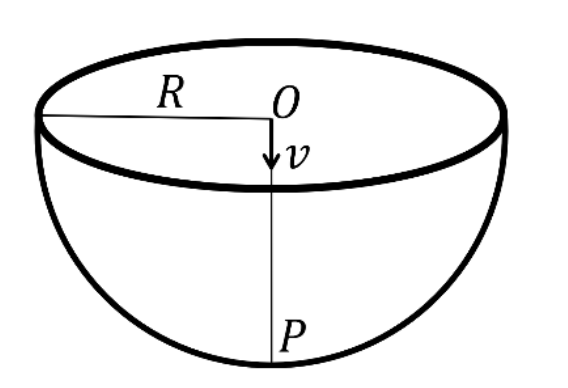
\includegraphics[width=\linewidth]{zhang_hemisphere.png}
\end{column}
\end{columns}
\[
 \varphi_P-\varphi_O=\frac{\sigma R}{2\epso}(\sqrt2-1).
\]
note：环带电量 $2\pi\sigma R^2\sin\theta\,\dd\theta$，弦长 $2R\sin(\theta/2)$。$\sin\theta=2\sin(\theta/2)\cos(\theta/2)$，故被积函数为 $\cos(\theta/2)$。
\src{2025秋基础物理学3期中考试A卷-张志财.pdf，PDF第4页，计算题2；答案PDF第3--4页。}
\end{frame}

\begin{frame}{e.g.1.2油滴的荷质比}
以碗底为重力势能的零点。从 $O$ 到 $P$ 下降的高度是 $R$，油滴在 $P$ 点速度为零：
\[
 \frac12 mv^2+mgR+q\varphi_O=q\varphi_P.
\]
\[
 \boxed{\frac qm
 =\frac{2\epso\left(gR+v^2/2\right)}{\sigma R(\sqrt2-1)}}.
\]
$\sigma>0$ 时碗底电势更高。油滴带正电，下落过程中电势能增加，静电力做负功，初动能和重力势能的减少都转成电势能。

式中有两处 $R$。电势里的 $R$ 是球面半径，用来算弦长和面积；能量式里的 $R$ 是下降高度。重力项 $mgR$ 不能再代进电势公式里约掉。
\src{2025秋基础物理学3期中考试A卷-张志财.pdf，计算题2；答案PDF第3--4页。}
\end{frame}

\begin{frame}{静电场边值关系}
在分界面上取扁柱体，由高斯定理，法向分量的跃变等于面电荷：
\[
 \hat{\vct n}\cdot(\vct E_2-\vct E_1)=\frac{\sigma}{\epso}.
\]
$\hat{\vct n}$ 从第 1 侧指向第 2 侧。其中 $\sigma$ 是界面上的全部面电荷。

再取贴在界面两侧的扁回路，由环路定理，切向分量连续，有：
\[
 \hat{\vct n}\times(\vct E_2-\vct E_1)=0.
\]
note：这一关系在导体和介质中适用，注意导体内部电场=0即可
\src{基础物理学(3)-电磁学部分教材.pdf，第2.7节；电磁学讲义\_20251125（张志财）.pdf，第3、4章的界面关系。}
\end{frame}

\begin{frame}{静电场中的导体}
静电平衡时，导体内电场为零，整块导体是等势体，电荷分布在表面。表面外侧的电场垂直于表面，
\[
 E_t=0,\qquad \epso E_n=\sigma,
\]
$\hat{\vct n}$ 指向导体外部。
note1：可以理解为切向电场如果不为零，电荷还会沿表面移动。\\

note2:空腔的内壁总感应电荷可以用导体内包围空腔的高斯面来求。导体内场为零，所以内壁总电荷等于腔内电荷的负值。\\

note3：孤立导体边界总电荷给定，接地导体边界电势$\varphi=0$给定，分别对应唯一性定理里的两类边界条件。
\src{DC2(理科).pdf，PDF第1--25页；电磁学讲义\_20251125（张志财）.pdf，PDF第67--76页，第3.1--3.2节。}
\end{frame}

\begin{frame}{唯一性定理}
导体上的电荷分布与电场互相决定，会导致思考与计算非常困难。一般的做法是把导体内部从求解区域里除掉，只求解剩下的空间，然后把导体当做边界条件。\\
由静电场唯一性定理：区域内电荷分布已经给定时，再给出下列边界条件之一，电势就唯一确定。电势可以差一个常数，电场则完全确定。
\begin{enumerate}
\item 给定边界上各处的电势。
\item 边界是等势面，并且给定面电荷密度，或给定每块导体的总电荷。
\item 前两种混合。
\end{enumerate}
因此，只要构造出的电势满足泊松方程和这些边界条件，它就是静电场的解。

e.g.静电屏蔽中，空腔的边界条件只由腔内电荷和内壁总电荷决定，腔外电荷改变不了它，也就改变不了腔内的场。导体接地时，外表面的边界条件是电势为零，腔内电荷的多少也不影响腔外的场。
\src{电磁学讲义\_20251125（张志财）.pdf，PDF第77--80页，第3.3节，定理3.1。}
\end{frame}

\begin{frame}{电像法}
在待求区域的外面放一个或几个假想电荷，称为镜像电荷。只要满足以下条件：
\begin{enumerate}
\item 镜像电荷不进入待求区域，区域内原有的电荷分布不变。
\item 真实电荷与镜像电荷合在一起，使导体表面成为等势面，而且电势等于题目给定的值。
\end{enumerate}
这样得到的电势满足区域内的泊松方程和边界条件。由唯一性定理就是这个区域的解。
note1：求解电像法时必须注意区分“物理空间”和“镜像空间”，一个物理空间上的镜像电荷必须存在于与物理空间正交的镜像空间里，但其产生的电场只在物理空间中有意义\\
note2：求表面电荷仍用$\sigma=\epso E_n$，电场取这个区域里的解。求真实电荷受到的力，只用镜像电荷在它位置上产生的场。\\
note3:电像法本质是凑解要先知道哪种电荷分布能给出所需形状的等势面，所以只适合平面、球面等少数边界。
\src{电磁学讲义\_20251125（张志财）.pdf，PDF第80--82页，第3.4节；基础物理学(3)-电磁学部分教材.pdf，第2.8节。}
\end{frame}

\begin{frame}{接地导体平面}
点电荷 $q$ 在无限大接地导体平面上方，距离为 $d$，平面电势为零。待求区域是平面上方。

在平面下方对称位置放镜像电荷 $-q$。等量异号的两个点电荷，中垂面电势为零，正好与接地平面重合，镜像电荷又在区域外面。上半空间的电势就是
\[
 \varphi=\frac{1}{4\pi\epso}\left(
 \frac{q}{R_+}-\frac{q}{R_-}\right),
\]
$R_+$、$R_-$ 分别是到 $q$ 和到 $-q$ 的距离。

平面上的感应电荷由外侧法向电场给出，
\[
 \sigma=-\frac{qd}{2\pi(r^2+d^2)^{3/2}}.
\]
对整个平面积分，总感应电荷等于 $-q$。正电荷把负电荷吸到近侧，密度在垂足处最大。
\src{电磁学讲义\_20251125（张志财）.pdf，PDF第81--82页，例3.5；基础物理学(3)-电磁学部分教材.pdf，例2.12。}
\end{frame}

\begin{frame}{镜像电荷的受力}
$q$ 受到的力等于镜像电荷 $-q$ 对它的库仑力。两者相距 $2d$，
\[
 F_d=-\frac{q^2}{16\pi\epso d^2}.
\]
$d$ 增大的方向离开平面，负号表示吸向平面。计算力时用镜像电荷的场，不再乘 $1/2$。

能量不能把 $q$ 和 $-q$ 当成两个真实点电荷。两个真实点电荷的相互作用能是 $-q^2/(8\pi\epso d)$，那是把两个电荷都从无穷远搬来的功。现在 $-q$ 是假想的，平面上的感应电荷随着 $q$ 一起产生。

对真实电荷只取一半：
\[
 W=\frac12 q\varphi_{\text{镜像}}
 =-\frac{q^2}{16\pi\epso d}.
\]
$\varphi_{\text{镜像}}$ 是 $-q$ 在 $q$ 处产生的电势。把 $q$ 从无穷远缓慢移到 $d$，外力与电场力平衡，外力做的功也是这个值。\alert{能量有 $1/2$，力没有 $1/2$。}
\src{电磁学讲义\_20251125（张志财）.pdf，例3.5；2025秋基础物理学3期中考试A卷-张志财.pdf，填空6，答案为 $-q^2/(16\pi\epso d)$。}
\end{frame}

\begin{frame}{导体球}
点电荷 $q$ 到球心的距离为 $a$，导体球半径为 $R$。两个异号、电量不相等的点电荷，零电势面是一个球面，球面把它们隔开。由此确定镜像电荷。

接地时，在球心与 $q$ 的连线上、离球心 $b=R^2/a$ 处放
\[
 q'=-\frac{R}{a}q.
\]
待求的那一侧只用 $q$ 和 $q'$。球外问题中 $q'$ 在球内；空腔问题中电荷在球内，$q'$ 就放到球外。球面上总感应电荷等于 $q'$。

球不接地、原来又不带电时，球面仍是等势面，但电势不一定为零，总电荷必须为零。再在球心放 $q''=(R/a)q$。它在球面上的电势是常数，不破坏等势，又与 $q'$ 抵消。这就是唯一性定理要求的“给定总电荷”。

$q$ 受到的力只来自镜像电荷。接地球把它吸向球心。孤立的中性球上，球心处的同号镜像向外推，球内的异号镜像向里拉，总效果仍是吸引。
\src{电磁学讲义\_20251125（张志财）.pdf，PDF第83--86页，例3.7。}
\end{frame}

\begin{frame}{电介质}
电介质在电场中会被极化。无极分子的正负电荷中心被拉开，有极分子的电矩转向电场方向，内部产生偶极子分布。宏观上用极化强度 $\vct P$ 表示，它等于单位体积内分子电偶极矩的矢量和，单位与面电荷密度相同。

极化电荷由 $\vct P$ 决定。$\hat{\vct n}$ 从介质指向外部，
\[
 \rho_b=-\nabla\cdot\vct P,\qquad
 \sigma_b=\vct P\cdot\hat{\vct n}.
\]
$\vct P$ 均匀时，内部正负电荷首尾相接，体电荷为零，电荷只出现在表面。$\vct P$ 沿外法向穿出的地方出现正的束缚面电荷。

各向同性线性介质中，极化与介质内的总电场成正比：
\[
 \vct P=\epso\chi_e\vct E,\qquad \chi_e>0.
\]
$\chi_e$ 是电极化率。注意这里的 $\vct E$ 是介质里的总场，包含极化电荷自己产生的场。
\src{电磁学讲义\_20251125（张志财）.pdf，PDF第89--95页，第4.1--4.2节；DC2(理科).pdf，PDF第47--65页。}
\end{frame}

\begin{frame}{电位移}
总电场的高斯定理右端包含全部电荷。极化电荷又由 $\vct P$ 决定，$\vct P$ 又依赖总电场，直接用 $\vct E$ 往往解不下去。于是我们引入电位移矢量：
\[
 \vct D=\epso\vct E+\vct P,
\]
这样在高斯定理积分中，把极化电荷移到左边：
\[
 \oiint_S\vct D\cdot\dd\vct S=Q_{f,\rm in},
 \qquad
 \nabla\cdot\vct D=\rho_f.
\]
$\vct D$ 的通量只和自由电荷有关，而一个介质体系的自由电荷是容易确定的。

在线性各向同性介质中 $\vct D=\varepsilon\vct E$，
\[
 \varepsilon=\varepsilon_r\epso=\epso(1+\chi_e),\qquad
 \vct P=\left(1-\frac{\epso}{\varepsilon}\right)\vct D.
\]
$\varepsilon$ 是介电常量，$\varepsilon_r$ 是相对介电常量。

环路定理只对$\vct E$成立。$\vct D$ 的环流一般不为零。只有介质分区均匀，并且分界面与等势面重合时，$\vct D$ 才和真空中的 $\epso\vct E$ 满足同一组方程。
\src{电磁学讲义\_20251125（张志财）.pdf，PDF第98--102页，第4.3节。}
\end{frame}

\begin{frame}{电介质的边值关系}
$\hat{\vct n}$ 从介质 1 指向介质 2。界面上的自由面电荷为 $\sigma_f$ 时，
\[
 \hat{\vct n}\times(\vct E_2-\vct E_1)=0,
 \qquad
 \hat{\vct n}\cdot(\vct D_2-\vct D_1)=\sigma_f.
\]
电势仍然连续。线性介质中，第二条就是 $\varepsilon_2 E_{2n}-\varepsilon_1 E_{1n}=\sigma_f$。

没有自由面电荷时 $D_n$ 连续，$E_n$ 一般不连续。切向电场连续，$D_t=\varepsilon E_t$不一定连续。

净束缚面电荷为：
\[
 \sigma_b=(\vct P_1-\vct P_2)\cdot\hat{\vct n}.
\]
\src{基础物理学(3)-电磁学部分教材.pdf，PDF第76--77页，第2.7节；2025秋 A 卷选择4。}
\end{frame}

\begin{frame}{均匀极化球}
\begin{columns}[T,onlytextwidth]
\begin{column}{0.70\textwidth}
半径为 $R$ 的球，内部 $\vct P$ 是常矢量，球外为真空。体束缚电荷为零，表面
\[
 \sigma_b=P\cos\theta.
\]
余弦分布的面电荷在球内产生均匀场。由球面电势连续和 $E_r$ 的跃变，我们有，
\[
 \vct E_{\rm in}=-\frac{\vct P}{3\epso}.
\]
这个场与$\vct P$相反，称为退极化场。
\end{column}
\begin{column}{0.26\textwidth}
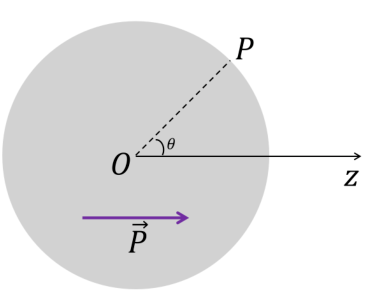
\includegraphics[width=\linewidth]{m1_uniform_polarization.png}
\end{column}
\end{columns}
总电偶极矩 $\vct p=(4\pi R^3/3)\vct P$。球外电场等效于这个球心处偶极子产生的场。
\[
 \vct E_{\rm out}
 =\frac{3(\vct p\cdot\hat{\vct r})\hat{\vct r}-\vct p}{4\pi\epso r^3}.
\]
\src{电磁学讲义\_20251125（张志财）.pdf，PDF第96页，例4.1；基础物理学(3)-电磁学部分教材.pdf，例2.5。}
\end{frame}

\begin{frame}{径向极化球}
\begin{columns}[T,onlytextwidth]
\begin{column}{0.72\textwidth}
球内$\vct P=f(r)\hat{\vct r}$，没有自由电荷，球外是真空。束缚电荷为
\[
 \rho_b=-\frac{1}{r^2}\frac{\dd}{\dd r}[r^2 f(r)],
 \qquad
 \sigma_b=f(R).
\]
取同心球面。自由电荷为零，对称性给出$D_r=0$，于是
\[
 \vct E_{\rm in}=-\frac{f(r)}{\epso}\hat{\vct r},
 \qquad
 \vct E_{\rm out}=0.
\]
note：这个结果只用了 $\vct D=\epso\vct E+\vct P$ 和自由电荷的高斯定理，不需要介质是线性的。
\end{column}
\begin{column}{0.24\textwidth}
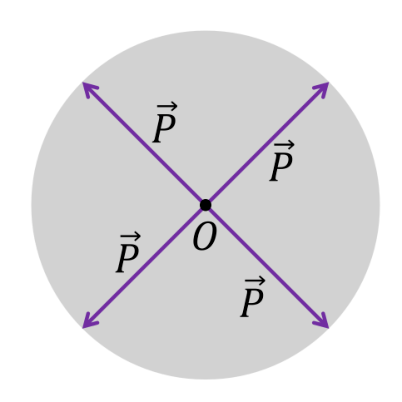
\includegraphics[width=\linewidth]{m1_radial_polarization.png}
\end{column}
\end{columns}
若 $f(r)=P$ 为常数，则 $\rho_b=-2P/r$，体电荷并不为零。球内的体电荷与球面电荷总量抵消，所以球外场为零。
\src{电磁学讲义\_20251125（张志财）.pdf，PDF第96--97页，例4.2；2025秋 A 卷填空2，答案 $\vct E=-f(r)\hat{\vct r}/\epso$。}
\end{frame}

\begin{frame}{匀强外场中的介质球}
均匀外场 $\vct E_0$ 中放入半径 $R$、介电常量 $\varepsilon$ 的线性介质球，球外为真空。均匀外场使球的极化也是均匀的，可以直接用上一节的退极化场：
\[
 \vct E_{\rm in}=\vct E_0-\frac{\vct P}{3\epso},
 \qquad
 \vct P=(\varepsilon-\epso)\vct E_{\rm in}.
\]
第二式里的电场是球内总场。联立后
\[
 \boxed{\vct E_{\rm in}=\frac{3\epso}{\varepsilon+2\epso}\vct E_0},
 \qquad
 \vct P=\frac{3\epso(\varepsilon-\epso)}{\varepsilon+2\epso}\vct E_0.
\]
球外是原来的均匀场加上球心偶极子的场，
\[
 \vct p=4\pi\epso R^3\frac{\varepsilon-\epso}{\varepsilon+2\epso}\vct E_0.
\]
这个势在球面上连续，法向 $\vct D$ 也连续，所以它就是唯一解。

$\varepsilon=\epso$ 时没有极化。$\varepsilon\to\infty$ 时球内场趋于零，$\vct p\to 4\pi\epso R^3\vct E_0$，回到不带电的导体球。导体球可以看成电像法中放在球心的偶极子。
\src{基础物理学(3)-电磁学部分教材.pdf，例2.8；电磁学讲义\_20251125（张志财）.pdf，习题3.3、例4.1。}
\end{frame}

\begin{frame}{双层球壳}
同心球形电容器，内导体半径 $a$，外导体内半径 $b$，介质在 $r=c$ 处分成两层，$a<c<b$，介电常量分别为 $\varepsilon_1$、$\varepsilon_2$。内导体自由电荷为 $Q$。

分界面是球面，与径向电场垂直，也与等势面重合。取同心球面，通量只由自由电荷决定，两层中
\[
 D_r=\frac{Q}{4\pi r^2},\qquad
 E_i=\frac{D_r}{\varepsilon_i}.
\]
介电常量大的一层场强小。两层电压相加，相当于串联：
\[
 C=4\pi\Big/
 \left[\frac1{\varepsilon_1}\left(\frac1a-\frac1c\right)
 +\frac1{\varepsilon_2}\left(\frac1c-\frac1b\right)\right].
\]
均匀介质内部 $\nabla\cdot\vct P=0$，束缚电荷只在表面上。$\vct P=(1-\epso/\varepsilon)\vct D$，
\[
 \sigma_b(a)=-P_1(a),\;
 \sigma_b(c)=P_1(c)-P_2(c),\;
 \sigma_b(b)=P_2(b).
\]
note：内表面的外法向指向球心，所以带负号。
\src{基础物理学(3)-电磁学部分教材.pdf，第2.7.5节，界面与等势面重合；张讲义习题4.3为同轴情形。}
\end{frame}

\begin{frame}{两个半球}
球形电容器内外半径 $a$、$b$，两导体带电 $\pm Q$。过球心的平面把介质分成两个半球，介电常量分别为 $\varepsilon_1$、$\varepsilon_2$。

分界面与径向电场平行。切向电场连续，两半球中的 $E$ 相同，都沿径向。一个闭合球面上，两侧电位移的通量相加等于 $Q$：
\[
 E=\frac{Q}{2\pi(\varepsilon_1+\varepsilon_2)r^2},\qquad
 D_i=\varepsilon_i E.
\]
两半球的 $D$ 不同，自由电荷在 $D$ 较大的一侧更多。电势差由同一个 $E$ 从 $a$ 积到 $b$，电容相当于并联：
\[
 C=\frac{2\pi(\varepsilon_1+\varepsilon_2)}{1/a-1/b}.
\]
$\varepsilon_1=\varepsilon_2=\varepsilon$ 时回到 $4\pi\varepsilon/(1/a-1/b)$。平界面上 $\vct P$ 与法向垂直，$\sigma_b=0$。
note：一般来说等势面平行界面方向时，D相等；等势面垂直界面方向时，E相等，但是本质还是电磁场的边界条件。
\src{基础物理学(3)-电磁学部分教材.pdf，例2.9，界面与电场线重合。}
\end{frame}

\begin{frame}{介质无穷大平面}
上半空间介电常量为 $\varepsilon_1$，下半空间为 $\varepsilon_2$。点电荷 $q$ 在界面上方距离 $d$ 处，界面没有自由电荷。

上半空间用 $q$ 和下侧对称位置的镜像 $q'$。下半空间用放在 $q$ 原位置的 $q''$。两组镜像不能放进同一个区域。
\[
 \varphi_1=\frac{1}{4\pi\varepsilon_1}
 \left(\frac{q}{R_+}+\frac{q'}{R_-}\right),
 \qquad
 \varphi_2=\frac{1}{4\pi\varepsilon_2}\frac{q''}{R_+}.
\]
电势连续、$D_z$ 连续，解出
\[
 q'=\frac{\varepsilon_1-\varepsilon_2}{\varepsilon_1+\varepsilon_2}q,\qquad
 q''=\frac{2\varepsilon_2}{\varepsilon_1+\varepsilon_2}q.
\]
$q$ 的受力只用 $q'$。$\varepsilon_2>\varepsilon_1$ 时电荷被吸向介质。$\varepsilon_2\to\infty$ 且 $\varepsilon_1=\epso$ 时回到接地导体平面。
\src{电磁学讲义\_20251125（张志财）.pdf，习题4.6；基础物理学(3)-电磁学部分教材.pdf，例2.13。}
\end{frame}

\begin{frame}{界面上的点电荷}
\begin{columns}[T,onlytextwidth]
\begin{column}{0.73\textwidth}
$z>0$ 为真空，$z<0$ 的相对介电常量为 $\varepsilon_r$。$q_1$ 在 $z=d$，$q_2$ 在 $z=-d$，界面没有自由面电荷。两个电荷分别做电像，再在各自区域里叠加。
\[
 q_1'=\frac{1-\varepsilon_r}{1+\varepsilon_r}q_1,\quad
 q_1''=\frac{2\varepsilon_r}{1+\varepsilon_r}q_1.
\]
对 $q_2$ 把两侧介电常量对调：
\[
 q_2'=\frac{\varepsilon_r-1}{\varepsilon_r+1}q_2,\quad
 q_2''=\frac{2}{1+\varepsilon_r}q_2.
\]
\end{column}
\begin{column}{0.24\textwidth}
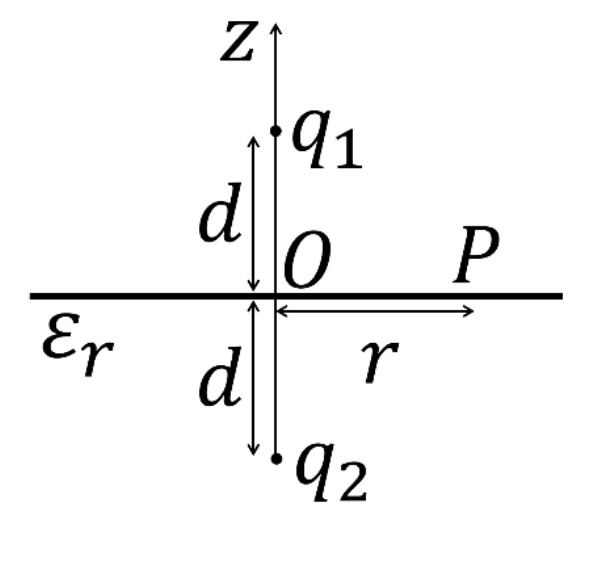
\includegraphics[width=\linewidth]{zhang_dielectric.png}
\end{column}
\end{columns}
上半空间用 $q_1$ 和位于 $z=-d$ 的 $q_1'+q_2''$。受力去掉 $q_1$ 自己的场，这两个电荷与它相距 $2d$，向上为正：
\[
 \boxed{F_{1z}
 =\frac{(1-\varepsilon_r)q_1^2+2q_1 q_2}
 {16\pi\epso(1+\varepsilon_r)d^2}}.
\]
$\varepsilon_r=1$ 时回到库仑力。$\varepsilon_r\to\infty$ 时 $q_1$ 的镜像趋于 $-q_1$，与接地平面一致。
\src{2025秋 A 卷计算题3；答案 PDF 第4--6页。单电荷模型为张讲义习题4.6。}
\end{frame}

\begin{frame}{界面上的束缚电荷}
束缚面电荷用介质一侧的电场。真空与介质的界面上，介质的外法向是 $+\hat{\vct z}$，
\[
 \sigma_b=P_z=\epso(\varepsilon_r-1)E_z(0^-).
\]
下半空间的电势用 $q_2$ 和位于 $z=d$ 的 $q_2'+q_1''$，分母里的介电常量是 $\varepsilon_r\epso$。在 $z=0$ 处，
\[
 E_z(0^-)=\frac{d\,(q_2-\varepsilon_r q_1)}
 {2\pi\epso\varepsilon_r(1+\varepsilon_r)L^3},
\]
$L=\sqrt{r^2+d^2}$。因此
\[
 \boxed{\sigma_b(r)
 =\frac{(q_1-q_2/\varepsilon_r)\,d\,(1-\varepsilon_r)}
 {2\pi(1+\varepsilon_r)(r^2+d^2)^{3/2}}}.
\]
$\varepsilon_r=1$ 时 $\sigma_b=0$。$q_2=0$ 时回到单个点电荷对着介质半空间的结果。

$q_1''$、$q_2''$ 只代表另一侧对这一侧的影响，不能把两侧的镜像电荷放进同一个库仑积分。
\src{2025秋 A 卷计算题3；答案 PDF 第4页，$\sigma'$ 与上式相同。}
\end{frame}

\begin{frame}{电势能}
外场已经给定、不因这个电荷而改变时，电荷在外场中的电势能是
\[
 W=q\varphi_{\text{外}}.
\]
电场力做的功等于电势能的减少。这里没有 $1/2$，$\varphi_{\text{外}}$ 也不包括该电荷自己的电势。产生外场的那些电荷，它们自己的能量不算在内。

电偶极矩 $\vct p$ 从负电荷指向正电荷。永久偶极子的大小和方向都固定时，它在外场中的电势能和力矩是
\[
 W=-\vct p\cdot\vct E_{\text{外}},
 \qquad
 \vct\tau=\vct p\times\vct E_{\text{外}}.
\]
匀强外场中合力为零，力矩使 $\vct p$ 转向电场方向。$W$ 仍然没有 $1/2$，因为外场是维持住的，不是和偶极子一起建立的。
\src{电磁学讲义\_20251125（张志财）.pdf，PDF第54--66页、第105页，第2.6节、第5.1节开头。}
\end{frame}

\begin{frame}{静电能}
电荷体系的静电能，等于把各电荷从无穷远处逐个搬到指定位置时，外力克服电场力做的功。

两个点电荷：先放好 $q_1$，不做功；再搬来 $q_2$，做功 $q_2\varphi_1$。
\[
 W=\frac{q_1 q_2}{4\pi\epso r}
 =\frac12(q_1\varphi_1+q_2\varphi_2).
\]
$\varphi_1$ 是另一个电荷在 $q_1$ 处的电势。$n$ 个点电荷写成 $W=\frac12\sum_i q_i\varphi_i$ 时，每一对相互作用出现两次，所以有 $1/2$。

连续分布时，电荷是逐渐加上去的，后加上的电荷面对已经升高的电势，
\[
 W=\frac12\int\rho\varphi\,\dd V
 =\frac{\epso}{2}\int E^2\,\dd V.
\]
有限大小的电荷分布上两个式子相等，并包含自能。点电荷自能发散，相互作用只保留电荷之间的项。
\src{电磁学讲义\_20251125（张志财）.pdf，PDF第105--109页，第5.1--5.2节，式(5.8)(5.9)(5.19)。}
\end{frame}

\begin{frame}{有介质时的能量}
搬动的是自由电荷，极化随之一起建立。电动力学里，元功是
\[
 \delta W=\int\vct E\cdot\delta\vct D\,\dd V.
\]
线性介质 $\vct D=\varepsilon\vct E$，积分后
\[
 W=\frac12\int\vct D\cdot\vct E\,\dd V
 =\frac12\int\rho_f\varphi\,\dd V.
\]
$\varphi$ 含自由电荷和极化电荷。铁电体不能用这个 $1/2$。$Q^2/(2C)$ 和 $CU^2/2$ 都是这个 $W$。

用 $\vct D=\epso\vct E+\vct P$ 拆开，
\[
 W=\int\frac{\epso E^2}{2}\,\dd V
 +\int\frac{\vct P\cdot\vct E}{2}\,\dd V.
\]
前一项等于对全部电荷作 $\frac12\int\rho\varphi\,\dd V$。后一项来自建立极化。中文教材对这两项的叫法并不一致，就不要纠结语言细节了。
\src{电磁学讲义\_20251125（张志财）.pdf，第5.3节，式(5.36)(5.39)(5.40)。电动力学中元功为 $\vct E\cdot\delta\vct D$。}
\end{frame}

\begin{frame}{偶极子的能量}
$\displaystyle\int\frac{\vct P\cdot\vct E}{2}\,\dd V$ 是上一页 $W$ 的第二项。永久偶极子的势能另写。

$\vct p$ 固定、外场由外界维持时，
\[
 W=-\vct p\cdot\vct E_{\text{外}}.
\]
这里没有 $1/2$。

诱导偶极子 $\vct p=\alpha\vct E$ 是场逐渐拉出来的。拉开电荷贡献 $\vct p\cdot\vct E/2$，与外场相互作用是 $-\vct p\cdot\vct E$，合起来
\[
 W=-\frac12\vct p\cdot\vct E=-\frac12\alpha E^2.
\]
电容器里储存多少能，用 $\frac12\int\vct D\cdot\vct E\,\dd V$。偶极子趋向强场还是弱场，用这里的 $W$：永久偶极子是 $-\vct p\cdot\vct E$，诱导偶极子是 $-\alpha E^2/2$。两处都是强场更低。
\src{电磁学讲义\_20251125（张志财）.pdf，式(5.42)--(5.45)。}
\end{frame}

\begin{frame}{电容}
两个导体分别带电 $+Q$、$-Q$，电势差为 $U=\varphi_+-\varphi_-$。电容定义为
\[
 C=\frac QU.
\]
电容只由几何形状和介质决定，表示同样的电势差下能储存电荷的能力；在同样的电势下，储存的能量 $CU^2/2$ 也更多。电荷固定时，能量是 $Q^2/(2C)$，$C$ 大则能量小。

求解电容的方法是假设法，先假设带有一定的电荷或具有一定的电势，求 $\vct D$ 或 $\vct E$，再沿电场积分得到 $U$。一些常见的结果有：
\[
 C_{\text{平板}}=\frac{\varepsilon S}{d},\qquad
 C_{\text{球}}=4\pi\varepsilon\frac{ab}{b-a},\qquad
 C_{\text{同轴}}=\frac{2\pi\varepsilon l}{\ln(b/a)}.
\]
电容的串并联行为可以将1/c与R类比
\src{电磁学讲义\_20251125（张志财）.pdf，PDF第114--118页，第5.4节。2025秋 A 卷选择6的答案是 A、C。}
\end{frame}

\begin{frame}{能量法求力}
设 $x$ 是介质插入的深度，$x$ 增大表示介质更进入电容器。$F_x$ 是电场对介质的力。

断开电源时 $Q$ 不变，没有能量从电源进来。电场力做正功，静电能减少：
\[
 F_x=-\left(\frac{\partial W}{\partial x}\right)_Q
 =\frac{Q^2}{2C^2}\frac{\dd C}{\dd x}.
\]
接在恒压电源上时 $U$ 不变。电源做功 $U\dd Q$，其中一部分成为静电能，其余是电场对介质做的功：
\[
 U\dd Q=\dd W+F_x\dd x.
\]
由 $\dd Q=U\dd C$、$\dd W=\frac12 U^2\dd C$，
\[
 F_x=\frac12 U^2\frac{\dd C}{\dd x}
 =+\left(\frac{\partial W}{\partial x}\right)_U.
\]
两个式子的符号不同，是因为 $Q$ 不变时能量随 $C$ 增大而减小，$U$ 不变时能量随 $C$ 增大而增大。$\dd C/\dd x>0$ 时都有 $F_x>0$，介质都被吸进去。拉出介质时，外力与 $F_x$ 反向。
\src{DC3(理科).pdf，PDF第1--34页；2025秋 A 卷选择9，恒压插入时介质受吸引力。}
\end{frame}

\begin{frame}{e.g.2.1能量法求抽出电容器介质板}
平行板长 $l$、宽 $b$、间距 $d$。介质厚度等于 $d$，介电常量为 $\varepsilon$，已经插入深度 $x$。忽略边缘对电容数值的影响，
\[
 C=\frac{\varepsilon bx}{d}+\frac{\epso b(l-x)}{d},
 \qquad
 \frac{\dd C}{\dd x}=\frac{(\varepsilon-\epso)b}{d}.
\]
两块极板是等势体，介质区和空气区的电势差相同，相当于并联。
\[
 F_x=
\begin{cases}
\dfrac{Q^2}{2C^2}\dfrac{(\varepsilon-\epso)b}{d}, & Q\ \text{不变},\\[10pt]
\dfrac{U^2}{2}\dfrac{(\varepsilon-\epso)b}{d}, & U\ \text{不变}.
\end{cases}
\]
$U$ 不变时 $E=U/d$ 不随 $x$ 改变，$F_x$ 是常数。$Q$ 不变时 $C$ 随插入增大，$E=Q/(Cd)$ 变小，吸力也变小。

$Q$ 不变，把板拉出：$C$ 减小，$W=Q^2/(2C)$ 增大，增加的能量等于外力做的功。

$U$ 不变，把板拉出：$W=CU^2/2$ 减小，外力仍然做正功。电荷流回电源，电源增加的能量等于外力的功加上电容器减少的静电能。
\src{由虚功原理与平行板电容公式计算。恒压时介质被吸入，与 2025 秋 A 卷选择9一致。}
\end{frame}

\begin{frame}{e.g.2.2电压强法求抽出电容器介质板}
介质从侧面插入时，端面与极板垂直，板间电场与这个端面平行。端面上 $\vct P$ 的法向分量为零，$\sigma_b=0$，不能写成 $\sigma_b E$。吸力来自边缘处的电场对极化电荷的作用，合起来相当于一个压强
\[
 p=\frac12(\varepsilon-\epso)E^2.
\]
方向指向空气一侧，也就是把介质拉进电容器。端面面积为 $bd$，
\[
 F_x=p\,bd=\frac12(\varepsilon-\epso)E^2\,bd.
\]
两区电势差相同，$E=U/d$。代入以后就是 $U$ 不变时的虚功结果。再写 $U=Q/C$，就得到 $Q$ 不变时的结果。同一种压强，对应两种约束下的同一个力。


\src{与上一页的 $\dd C/\dd x$ 对照。压强公式用于电场与介质端面平行的情形。}
\end{frame}

\begin{frame}{电偶极子}
两个点电荷 $\pm q$ 相距 $l$，$\vct p=q\vct l$，方向从负电荷指向正电荷。$r\gg l$ 时
\[
 \varphi=\frac{\vct p\cdot\hat{\vct r}}{4\pi\epso r^2},\qquad
 \vct E=\frac{3(\vct p\cdot\hat{\vct r})\hat{\vct r}-\vct p}{4\pi\epso r^3}.
\]
轴线上场强为 $2p/(4\pi\epso r^3)$，中垂面上场强与 $\vct p$ 反向，大小是轴上的一半。介质球和导体球的球外场都用这个式子。

永久偶极子的 $\vct p$ 固定。匀强场中合力为零，力矩 $\vct\tau=\vct p\times\vct E$ 使 $\vct p$ 转向电场。非匀强场中的力见下一页。计算 $\vct E$ 时去掉偶极子自己的场。
\src{DC1(理科).pdf，PDF第19--30页；电磁学讲义\_20251125（张志财）.pdf，PDF第39--43页。}
\end{frame}

\begin{frame}{偶极子的受力}
电磁学里按势能求梯度，$\vct E$ 用外场，下面两种算法可以把题目做对。

永久偶极子，$\vct p$ 为常矢量，且 $\nabla\times\vct E=0$：
\[
 \vct F=(\vct p\cdot\nabla)\vct E
 =\nabla(\vct p\cdot\vct E)
 =-\nabla W,
 \qquad
 W=-\vct p\cdot\vct E.
\]
$\vct p$ 与 $\vct E$ 同向时，力指向强场。

诱导偶极子 $\vct p=\alpha\vct E$，$\alpha>0$：
\[
 W=-\frac12\alpha E^2,
 \qquad
 \vct F=\nabla\!\left(\frac12\alpha E^2\right)
 =(\vct p\cdot\nabla)\vct E.
\]
仍指向强场。若先写 $W=-\vct p\cdot\vct E$，再代入 $\vct p=\alpha\vct E$，力大一倍。

严格的力的求解方法要用电动力学。真空中取包围物体的闭合面，合力等于 Maxwell 应力张量在这个面上的积分。介质内的力密度可以写成 $(\vct P\cdot\nabla)\vct E$，也可以写成 $-\frac12 E^2\nabla\varepsilon$ 再加上形变引起的压强。两者差一个应力的散度，并进内部应力以后，整块物体的合力相同。虚功给出的就是这个合力。
\src{电磁学中的虚功与 $(\vct p\cdot\nabla)\vct E$。严格计算用真空闭合面上的 Maxwell 应力张量。}
\end{frame}

\begin{frame}{稳恒电流}
稳恒时电荷密度不随时间变化，任意闭合曲面的净电流为零：
\[
 I=\int_S\vct J\cdot\dd\vct S,\qquad
 \nabla\cdot\vct J=0,\qquad
 \vct J=\sigma\vct E.
\]
导体内可以有电场，这与静电平衡不同。电场仍然满足环路定理，$\vct E=-\nabla\varphi$。

均匀导体中 $\sigma$ 是常数，由 $\nabla\cdot\vct J=0$ 得到 $\nabla\cdot\vct E=0$。电势满足拉普拉斯方程，和无自由电荷的均匀介质相同。

分界面上，电荷不再积累，所以 $J_n$ 连续；切向电场仍然连续。这与介质界面上 $\sigma_f=0$ 时 $D_n$ 连续、$E_t$ 连续是同一组要求。焦耳功率密度为 $\vct J\cdot\vct E$，能量由电源持续供给。
\src{DC4(理科).pdf，PDF第1--15页；基础物理学(3)-电磁学部分教材.pdf，第4.1--4.2节。}
\end{frame}

\begin{frame}{电流场与静电场}
均匀线性介质里 $\vct D=\varepsilon\vct E$，均匀导体里 $\vct J=\sigma\vct E$。没有自由电荷时 $\nabla\cdot\vct D=0$，稳恒时 $\nabla\cdot\vct J=0$。两者满足同一类方程，边界上法向分量连续、切向电场连续。因此几何相同的解可以互相改写：把 $\vct D$ 换成 $\vct J$，把 $\varepsilon$ 换成 $\sigma$。

同一几何下，电容和电导只差这个材料常数。漏电电容器
\[
 RC=\frac{\varepsilon}{\sigma},\qquad
 Q(t)=Q(0)\e^{-\sigma t/\varepsilon}.
\]
两个同心球面之间充满均匀介质，内半径 $a$、外半径 $b$ 时，
\[
 C=\frac{4\pi\varepsilon}{1/a-1/b},\qquad
 R=\frac{1}{4\pi\sigma}\left(\frac1a-\frac1b\right).
\]
截面沿电流方向缓慢变化时，把导体切成串联薄片，
\[
 R=\int\frac{\dd l}{\sigma A(l)}.
\]
圆台导线两端半径 $a$、$b$，长 $l$，得到 $R=l/(\pi\sigma ab)$。$b\to a$ 时回到圆柱电阻 $l/(\pi\sigma a^2)$。
\src{DC4(理科).pdf，PDF第16--21页；基础物理学(3)-电磁学部分教材.pdf，习题4.3、4.5。}
\end{frame}

\section{静磁场}
\gdef\coursepart{静磁场与磁介质}

\begin{frame}{静磁场}
磁场是存在于运动电荷或电流周围的、能传递运动电荷与电流之间相互作用的物理场。静磁场是指稳恒电流产生的、各处大小与方向都不变的磁场，用磁感应强度 $\vct B$ 描述。
静磁场的基本性质：散度定理（高斯定理，磁感应线闭合），环路定理（安培环路定理，环流由电流决定）。

几类静磁场问题的一般方法：\\
（1）利用安培环路定理/毕奥--萨伐尔定律与磁矢势求解 $\vct B$\\
（2）磁力与磁矩：洛伦兹力、安培力，以及磁矩的力矩、能量和受力\\
（3）介质问题：引入 $\vct H$，利用本构方程和边值关系求解；$\vct H$ 对应静电场的 $\vct E$\\
（4）磁路：铁芯把磁通集中成回路时，用磁路定理
\src{张讲义第6、7章；基础物理学(3)-电磁学部分教材，第5、6章；DC5、DC6。}
\end{frame}

\begin{frame}{磁感应强度}
只有静磁场时，运动电荷受力
\[
 \vct F=q\vct v\times\vct B.
\]
$\vct B$ 叫做磁感应强度。$\vct v$ 与 $\vct B$ 垂直时，$B=F/(|q|v)$。正电荷受力沿 $\vct v\times\vct B$，由此确定 $\vct B$ 的指向。单位是特斯拉，$\unit{1\,T=1\,N/(A\cdot m)}$。

$\vct B$ 是场本身的性质，与探测电荷的电量和速度无关。速度与 $\vct B$ 平行时磁力为零。静止电荷不受磁力。

洛伦兹以带电电流元的形式表现可以得到安培力 $\dd\vct F=I\dd\vct l\times\vct B$。电流元中的电荷以速度 $\vct v$ 运动，即$I\dd\vct l=\dd q\,\vct v$
\src{基础物理学(3)-电磁学部分教材，第5.1.3节，式(5.1.6)；张讲义，式(6.123)--(6.125)。}
\end{frame}

\begin{frame}{高斯定理}
在静磁场中取任何一个闭合面，其净磁通为零。由此可以推出磁场没有任何一个源/汇，磁感应线闭合，没有起点和终点：
\[
 \oiint_S\vct B\cdot\dd\vct S=0,
 \qquad
 \nabla\cdot\vct B=0.
\]

穿过开口曲面的磁通定义为
\[
 \Phi_B=\iint_S\vct B\cdot\dd\vct S.
\]
正负由所选法向决定，法向一般回路绕向配成右手关系。
如果假设存在磁单极子，磁高斯会被改写成和电高斯一致的形式。
\src{张讲义，PDF128--129；DC5，PDF26--31；教材第5.4节。}
\end{frame}

\begin{frame}{安培环路定理}
真空中，电流稳恒时
\[
 \oint_L\vct B\cdot\dd\vct l=\muo I_{\rm enc},
 \qquad
 \nabla\times\vct B=\muo\vct J.
\]
$I_{\rm enc}$ 是回路套住的全部电流。

note1：这里的I代表着全部的电流，有磁介质时，上式右端还要加上磁化电流。\\
note2：安培环路定理必须对“物理的”电流作用，即这一电流必须本身构成了完整的回路（含无穷远），对于部分电流作安培环路定理会得到错误的结果。\\
note3：在体系具有一定对称性时，用安培环路定理可以简化磁场的运算

\src{张讲义，PDF135--136；DC5，PDF26--35；教材第5.4节。}
\end{frame}

\begin{frame}{毕奥--萨伐尔定律}
真空中，稳恒电流元 $I\dd\vct l'$ 在场点如下大小与方向的电场
\[
 \dd\vct B=\frac{\muo}{4\pi}
 \frac{I\dd\vct l'\times(\vct r-\vct r')}{|\vct r-\vct r'|^3}.
\]
$\vct r'$ 是源点，$\vct r$ 是场点。叉乘里的矢量从源点指向场点。全部电流的场把上式叠加起来。

体电流、面电流把 $I\dd\vct l'$ 换成 $\vct J\dd V'$、$\vct K\dd S'$：
\[
 \vct B(\vct r)=\frac{\muo}{4\pi}\iiint
 \frac{\vct J(\vct r')\times(\vct r-\vct r')}{|\vct r-\vct r'|^3}\,\dd V'.
\]


note：计算时一般先用对称性消去互相抵消的分量，e.g.直导线只有垂直于导线的分量，圆电流的轴线只有下轴向分量。
\src{张讲义，PDF124，定律6.1，式(6.18)--(6.19)；DC5，PDF8--10。}
\end{frame}

\begin{frame}{有限长直导线}
\begin{columns}[T,onlytextwidth]
\begin{column}{0.72\textwidth}
场点到导线的垂直距离为 $a$。$\theta$ 是电流方向与“电流元到场点连线”的夹角，两端的角为 $\theta_1$、$\theta_2$。
\[
 B=\frac{\muo I}{4\pi a}(\cos\theta_1-\cos\theta_2).
\]
无限长时 $\theta_1=0$、$\theta_2=\pi$，
\[
 B=\frac{\muo I}{2\pi a}.
\]
半无限长时 $\theta_2=\pi/2$，$B=\muo I/(4\pi a)$。方向由电流与垂线的右手螺旋确定。
\end{column}
\begin{column}{0.24\textwidth}
\centering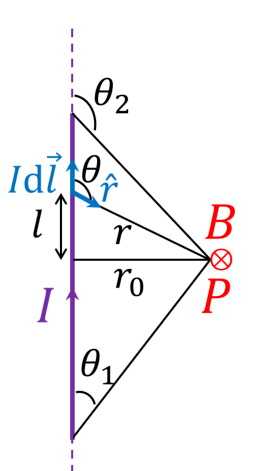
\includegraphics[height=200pt]{m2_finite_wire.png}
\end{column}
\end{columns}
$\theta$ 从电流的去向量起。电流上游的一端 $\theta$ 是锐角，下游的一端是钝角，$\cos\theta_1-\cos\theta_2$ 为正。$a$ 是垂直距离，不是到端点的斜边。
\src{张讲义，PDF124--125，例6.1，式(6.22)--(6.24)；DC5，PDF11--13。}
\end{frame}

\begin{frame}{圆电流环}
\begin{columns}[T,onlytextwidth]
\begin{column}{0.62\textwidth}
半径 $R$ 的圆环，电流 $I$。轴上成对电流元的横向磁场抵消，只留下轴向分量。
\[
 B_z=\frac{\muo I R^2}{2(R^2+z^2)^{3/2}}.
\]
圆心处 $B=\muo I/(2R)$。$z\gg R$ 时
\[
 B_z\simeq\frac{\muo I R^2}{2z^3}=\frac{\muo m}{2\pi z^3}.
\]
磁矩 $\vct m=I\pi R^2\vct e_z$，方向由电流的右手螺旋确定。远处按 $1/z^3$ 衰减，和电偶极子相同。
\end{column}
\begin{column}{0.34\textwidth}
\centering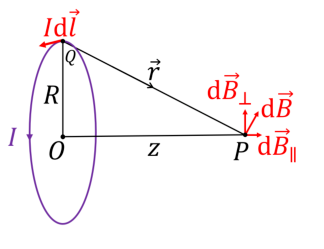
\includegraphics[width=\linewidth]{m2_ring.png}
\end{column}
\end{columns}
轴线公式要求场点在对称轴上。不在轴上时，横向分量不再成对抵消，要改用磁矢势，或在远处用磁偶极子的场。
\src{张讲义，PDF125，例6.2，式(6.27)--(6.31)；DC5，PDF14--16。}
\end{frame}

\begin{frame}{正多边形电流}
正 $N$ 边形通有电流 $I$，中心到每一条边的垂直距离为 $R$。

一条边的两端相对垂足各偏过 $\pi/N$。直导线公式里的两个端角是
\[
 \theta_{1,2}=\frac\pi2\mp\frac\pi N.
\]
代入后，这一条边在中心的场为
\[
 B_{\rm side}=\frac{\muo I}{2\pi R}\sin\frac\pi N.
\]
各边在中心处方向相同，
\[
 \boxed{B=\frac{N\muo I}{2\pi R}\sin\frac\pi N}.
\]
$N\to\infty$ 时 $\sin(\pi/N)\approx\pi/N$，得到 $B\to\muo I/(2R)$，就是半径为 $R$ 的圆电流在圆心的场。

$R$ 是内切圆半径，也就是中心到边的距离，不是中心到顶点的距离。极限若对不上圆电流，先检查用的是不是这个 $R$。
\src{2025秋基础物理学3期中考试A卷-张志财，PDF3，填空4；张讲义例6.1。}
\end{frame}

\begin{frame}{长直螺线管}
理想密绕螺线管，每单位长度 $n$ 匝，电流 $I$。无限长时，$\vct B$ 沿轴向，大小只与到轴的距离有关。

矩形回路的两条长边都在管外时，套住的电流为零，$\vct B$ 不随半径变化。无穷远处场为零，所以管外场为零。再把一条长 $l$ 的长边放进管内：
\[
 B_{\rm in}l=\muo(nl)I,
 \qquad
 \vct B_{\rm in}=\muo nI\,\vct e_z,
 \qquad
 \vct B_{\rm out}=0.
\]
管外这一步用了“无穷远处场为零”。有限长管只在 $L\gg R$、而且远离两个端口时能这样用。半无限长管的轴线上，端口处的场是 $\muo nI/2$。

密绕细螺绕环管内 $B=\muo NI/(2\pi r)$。环很细时 $n=N/(2\pi R)$，与长直螺线管相同。环外的环向场为零。
\src{张讲义，例6.4、例6.8；教材例5.6、例5.8；DC5，PDF35--39。}
\end{frame}

\begin{frame}{厚壁螺线管}
\begin{columns}[T,onlytextwidth]
\begin{column}{0.66\textwidth}
$R_1<s<R_2$ 的壁内有环向电流 $\vct J=J_0\vct e_\phi$，求全空间的 $\vct B$。

把壁拆成半径 $s$、厚度 $\dd s$ 的薄层。这一层的面电流是 $\dd K=J_0\dd s$，相当于 $nI=J_0\dd s$ 的无限长螺线管。螺线管只在内部有场，所以对半径为 $r$ 的场点
\[
 \dd B_z=\begin{cases}
 \muo J_0\dd s,&r<s,\\
 0,&r>s.
 \end{cases}
\]
只有位于场点外侧的电流层有贡献。
\end{column}
\begin{column}{0.30\textwidth}
\centering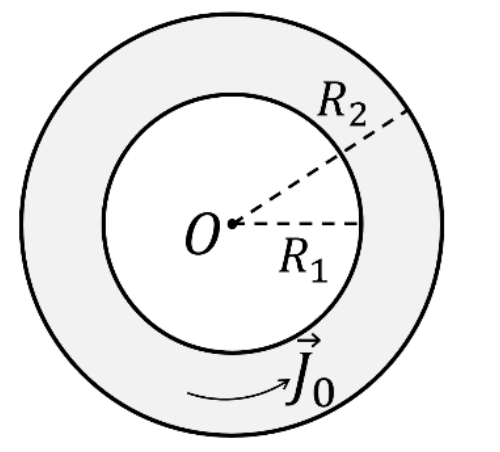
\includegraphics[width=\linewidth]{zhang_solenoid.png}
\end{column}
\end{columns}
积分下限随场点改变：内孔对全部壁积分，壁内只对 $s>r$ 的部分积分，壁外没有贡献。$J_0\dd s$ 的单位是 A/m，和面电流密度相同。
\src{2025秋 A 卷，PDF3，计算1；张讲义例6.4、例6.8。}
\end{frame}

\begin{frame}{壁内外的磁场}
\[
 B_z(r)=\begin{cases}
 \muo J_0(R_2-R_1),&r<R_1,\\[4pt]
 \muo J_0(R_2-r),&R_1<r<R_2,\\[4pt]
 0,&r>R_2.
 \end{cases}
\]
内孔的场是均匀的，大小等于 $\muo$ 乘壁的总面电流密度 $J_0(R_2-R_1)$。壁内场从内边界的值线性降到外边界的零。

在电流区内，$-\dd B_z/\dd r=\muo J_0$，与安培环路定理 $\nabla\times\vct B=\muo\vct J$ 一致。$r=R_1$ 和 $r=R_2$ 上没有额外的面电流，$B_z$ 在这两处都连续。若积分限写成从 $R_1$ 积到 $r$，壁内场会反号，方向就错了。
\src{2025秋 A 卷计算1；配套答案，PDF2。}
\end{frame}

\begin{frame}{磁矢势}
$\nabla\cdot\vct B=0$，而任一矢量的旋度再取散度恒为零，所以存在矢量 $\vct A$，使
\[
 \vct B=\nabla\times\vct A.
\]
$\vct A$ 称为磁矢势。

$\vct A$ 不唯一。换成 $\vct A+\nabla\chi$ 做规范变换之后旋度不变，$\vct B$ 也不变。只给定旋度还定不下 $\vct A$，还要规定它的散度，这就是取规范。

$\vct A$ 沿闭合曲线的积分等于穿过该曲线的磁通：
\[
 \oint_L\vct A\cdot\dd\vct l=\iint_S\vct B\cdot\dd\vct S=\Phi_B.
\]
毕奥--萨伐尔定律先做叉乘再积分。先积$\vct A$只做一次矢量积分，再取旋度。电流产生的 $\vct A$ 大体沿电流方向：直导线的 $\vct A$ 沿导线，圆电流的 $\vct A$ 沿环向。
\src{张讲义，第6.3节，式(6.108)；教材第5.5.1节，式(5.5.1)。}
\end{frame}

\begin{frame}{规范}
库仑规范：$\nabla\cdot\vct A=0$。用 $\nabla\times(\nabla\times\vct A)=\nabla(\nabla\cdot\vct A)-\nabla^2\vct A$，代入 $\nabla\times\vct B=\muo\vct J$，得到
\[
 \nabla^2\vct A=-\muo\vct J.
\]
在直角坐标系里，每个分量都是泊松方程，和电势满足的方程相同。电流稳恒、无穷远处 $\vct A$ 为零时，
\[
 \vct A(\vct r)=\frac{\muo}{4\pi}\iiint\frac{\vct J(\vct r')}{|\vct r-\vct r'|}\,\dd V'.
\]
稳恒条件 $\nabla\cdot\vct J=0$ 保证这个解的散度为零。对它取旋度，就回到毕奥--萨伐尔定律。

洛伦兹规范是
\[
 \nabla\cdot\vct A+\muo\epso\frac{\partial\varphi}{\partial t}=0.
\]
静磁场不随时间变化，上式同样回到 $\nabla\cdot\vct A=0$，方程和解都与库仑规范相同。场随时间变化以后，洛伦兹规范使矢势和电势各自满足波动方程。

e.g.匀强场$\vct B=B\vct e_z$可以取$\vct A=\frac12\vct B\times\vct r$等多种形式。场一直延伸到无穷远时，只要求散度为零，还不能把 $\vct A$ 唯一确定。
\src{张讲义，PDF137--138，式(6.109)--(6.112)；DC5，PDF44--47。静磁场中洛伦兹规范与库仑规范重合。}
\end{frame}

\begin{frame}{静磁场的边值关系}
$\hat{\vct n}$ 从第 1 侧指向第 2 侧。由高斯定理，法向分量连续：
\[
 \hat{\vct n}\cdot(\vct B_2-\vct B_1)=0.
\]
由环路定理，切向分量的跃变由面电流决定：
\[
 \hat{\vct n}\times(\vct B_2-\vct B_1)=\muo\vct K.
\]
这里的 $\vct K$ 是界面上的全部面电流。真空中它就是导线或电流片上的电流。

e.g.无限大均匀面电流两侧是均匀场，大小都是 $\muo K/2$，方向相反，并与电流垂直。密绕长螺线管的管壁可以看成这样的面电流，$K=nI$，管内 $\muo nI$、管外为零，两侧之差正好是 $\muo K$。

\src{由 $\nabla\cdot\vct B=0$ 与 $\nabla\times\vct B=\muo\vct J$ 得到；无限大电流片见教材例5.7，式(5.4.8)。}
\end{frame}

\begin{frame}{洛伦兹力}
\[
 \vct F=q(\vct E+\vct v\times\vct B).
\]
磁力与速度垂直，$\vct F_B\cdot\vct v=0$，不改变动能，只改变方向。

均匀磁场中，平行于 $\vct B$ 的速度分量不变。垂直分量作圆周运动，正、负电荷的回旋方向相反。
\[
 r_c=\frac{mv_\perp}{|q|B},\qquad
 \omega_c=\frac{|q|B}{m},\qquad
 T_c=\frac{2\pi m}{|q|B}.
\]
note：洛伦兹力是相对论下不变的，但是质量等参数需要做相对论变换。
\src{张讲义，第6.4节；教材第5.6节，式(5.6.7)--(5.6.10)；DC5，PDF49、56。}
\end{frame}

\begin{frame}{霍尔效应}
\begin{columns}[T,onlytextwidth]
\begin{column}{0.67\textwidth}
考虑这样的情景情景：电流向右，磁场垂直纸面向里，测得上极板高电势。

电场由高电势指向低电势，所以上极板到下极板的霍尔电场向下。横向达到平衡时，磁力与电场力抵消，
\[
 \vct E_H=-\vct v_d\times\vct B.
\]
由此得到漂移速度 $\vct v_d$ 向右，与电流同向，载流子带正电。若载流子带负电，同样的电流方向要求 $\vct v_d$ 向左，上极板会是低电势。
\end{column}
\begin{column}{0.29\textwidth}
\centering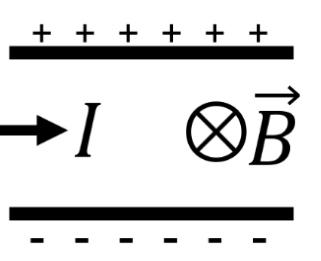
\includegraphics[width=\linewidth]{m2_hall_exam.png}
\end{column}
\end{columns}
单一载流子、厚度 $t$ 沿磁场方向时，
\[
 |U_H|=\frac{IB}{n|q|t},\qquad R_H=\frac{1}{nq}.
\]
$R_H$ 的符号与载流子的符号相同。
\src{2025秋 A 卷，PDF2，选择11；张讲义，PDF138--140；DC5，PDF49--52。}
\end{frame}

\begin{frame}{安培力}
电流元受力
\[
 \dd\vct F=I\dd\vct l\times\vct B,
 \qquad
 \vct F=I\int\dd\vct l\times\vct B.
\]
$\dd\vct l$ 沿电流方向。均匀磁场中，闭合导线的 $\int\dd\vct l=0$，合力为零。合力为零时仍可以有力矩，平面线圈的力矩由磁矩给出。

计算一段导线时，$\vct B$ 取该段所在处的外场。\\
e.g.1面电流自己两侧的场不连续，受力公式里要用两侧的平均值，不能把间断点上的值代进去。
e.g.2两根平行长直导线：电流同向相吸，反向相斥。距离为 $a$ 时，单位长度的力是 $\muo I_1 I_2/(2\pi a)$。
\src{张讲义，式(6.123)；教材第6.1节；DC5，PDF5--7。}
\end{frame}

\begin{frame}{导线受力}
\begin{columns}[T,onlytextwidth]
\begin{column}{0.66\textwidth}
均匀磁场只覆盖闭合导线的一段。沿电流方向，入场点为 $A$，出场点为 $B$。场外 $\vct B=0$，总力只来自场内这一段：
\[
 \vct F=I\int_A^B\dd\vct l\times\vct B
 =I(\vct r_B-\vct r_A)\times\vct B.
\]
若$\vct B$ 均匀，可以把它提出积分。积分 $\int_A^B\dd\vct l$ 只取决于两端，与场内导线弯曲形状无关。

两交点间距为 $w$，磁场垂直于导线所在平面时，$F=IBw$。
\end{column}
\begin{column}{0.30\textwidth}
\centering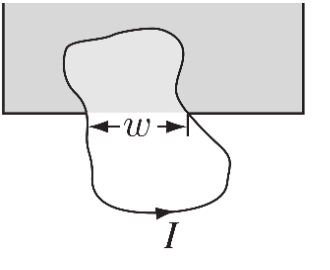
\includegraphics[width=\linewidth]{m2_force_exam.png}
\end{column}
\end{columns}
整环都在同一均匀场中时，$\vct r_B=\vct r_A$，合力为零。
\src{2025秋 A 卷，PDF2--3，选择12；DC5，PDF7，半圆导线受力。}
\end{frame}

\begin{frame}{磁矩}
平面线圈的面积为 $S$，法向与电流成右手关系：
\[
 \vct m=IS\vct n.
\]
均匀外场中，闭合线圈合力为零，力矩和能量为
\[
 \vct\tau=\vct m\times\vct B,
 \qquad
 U=-\vct m\cdot\vct B.
\]
电流保持不变时用这个能量。$\vct m$ 与 $\vct B$ 同向时能量最低，反向时最高。

线圈很小，磁矩不随位置改变，且线圈所在处没有电流时，磁矩受力为
\[
 \vct F=\nabla(\vct m\cdot\vct B).
\]
它和 $(\vct m\cdot\nabla)\vct B$ 相同。线圈所在处有电流时，回到安培力重新积分。

远处的场和电偶极子对应。磁矩 $\vct m$ 在 $r$ 远大于线圈尺寸处，
\[
 \vct B=\frac{\muo}{4\pi r^3}\bigl[3(\vct m\cdot\hat{\vct r})\hat{\vct r}-\vct m\bigr].
\]
\src{张讲义，式(6.121)--(6.122)，例6.10；教材式(6.1.9)、(6.1.10)。}
\end{frame}

\begin{frame}{e.g.3.1旋转带电圆盘}
半径 $R$ 的圆盘均匀带电 $q$，以角速度 $\vct\omega=\omega\vct e_z$ 绕轴转动。面密度 $\sigma=q/(\pi R^2)$。

半径 $r$、宽度 $\dd r$ 的环带，电量 $\dd q=\sigma\,2\pi r\dd r$。转一圈的时间是 $2\pi/\omega$，对应的电流
\[
 \dd I=\sigma\omega r\,\dd r.
\]
$q>0$ 时电流沿转动方向，$q<0$ 时相反。

该环在圆心的场用圆电流公式，
\[
 \dd B_z=\frac{\muo\dd I}{2r}=\frac{\muo\sigma\omega}{2}\dd r.
\]
环带电量随 $r$ 增大，圆电流中心场中的 $1/r$ 正好抵消，等宽环带的贡献相同。
\[
 B_z=\frac{\muo\sigma\omega R}{2}=\frac{\muo q\omega}{2\pi R},
 \qquad
 \vct B_O=\frac{\muo q}{2\pi R}\vct\omega.
\]
总电荷和角速度固定时，中心磁场按 $1/R$ 减小。这个 $\vct B_O$ 是盘自己在圆心的场，不是外加场。
\src{张讲义习题6.10(1)；教材习题6.6；第六周作业，6.6。}
\end{frame}

\begin{frame}{e.g.3.2旋转带电圆盘}
每一环带的磁矩是电流乘环面积，方向都沿 $\vct\omega$（$q>0$）：
\[
 \dd m=\pi r^2\dd I=\pi\sigma\omega r^3\dd r.
\]
\[
 \vct m=\pi\sigma\omega\int_0^R r^3\dd r\,\vct e_z
 =\frac{q R^2}{4}\vct\omega.
\]
均匀外场 $\vct B_{\rm ext}$ 平行于盘面时，
\[
 \vct\tau=\vct m\times\vct B_{\rm ext},
 \qquad
 |\tau|=\frac{|q|\omega R^2 B_{\rm ext}}{4}.
\]
磁矩的被积函数带 $r^3$，外圈贡献大。中心磁场的被积函数是 $\dd r$，各圈一样。两个积分的权重不同，不能用中心磁场乘总面积去写磁矩。

力矩公式里的 $\vct B_{\rm ext}$ 是外加的均匀场。盘自己的场对总力矩没有贡献。
\src{张讲义习题6.10(2)，参考答案 PDF216；教材习题6.6。}
\end{frame}

\begin{frame}{磁化强度}
磁化强度是单位体积内分子磁矩的矢量和，
\[
 \vct M=\frac{\dd\vct m}{\dd V}.
\]
单位是 A/m。分子电流排列整齐以后，宏观上相当于一组磁化电流。$\hat{\vct n}$ 指向介质外部时，
\[
 \vct J'=\nabla\times\vct M,
 \qquad
 \vct K'=\vct M\times\hat{\vct n}.
\]
$\vct J'$ 的单位是 A/m$^2$，$\vct K'$ 的单位是 A/m。

\begin{columns}[T,onlytextwidth]
\begin{column}{0.48\textwidth}
\centering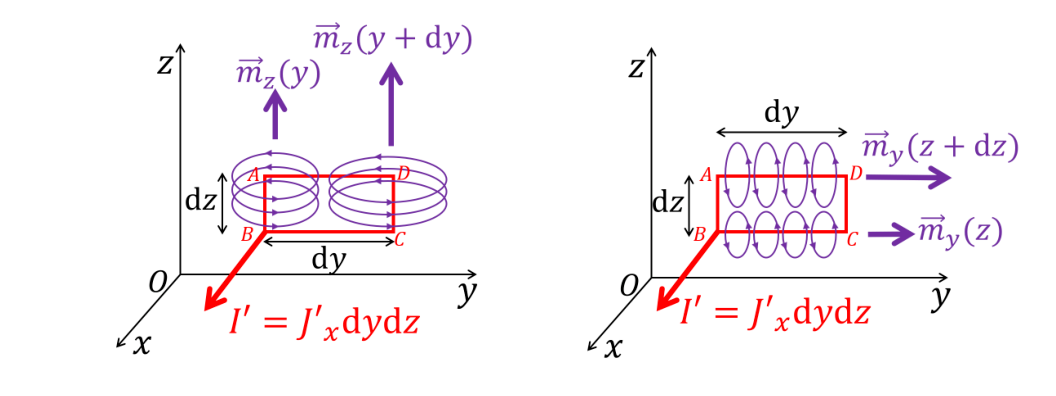
\includegraphics[width=0.92\linewidth]{m2_bound_bulk.png}
\end{column}
\begin{column}{0.48\textwidth}
$\vct M$ 均匀时，内部相邻分子电流首尾抵消，$\vct J'=0$，表面仍可以有 $\vct K'$。$\vct M$ 沿外法向没有贡献；平行于表面的分量留下环向面电流。
\end{column}
\end{columns}
磁化电流激发磁场、也受磁场作用，算法与传导电流相同。但是它不伴随电荷的宏观迁移，不会产生焦耳热。
\src{张讲义，式(7.2)、(7.12)；教材式(6.2.5)、(6.2.6)；DC6，PDF21--24。}
\end{frame}

\begin{frame}{磁场强度}
总电流是传导电流加磁化电流，$\nabla\times\vct B=\muo(\vct J_0+\nabla\times\vct M)$。定义
\[
 \vct H=\frac{\vct B}{\muo}-\vct M,
 \qquad
 \vct B=\muo(\vct H+\vct M),
\]
则
\[
 \oint_L\vct H\cdot\dd\vct l=I_{0,\rm enc},
 \qquad
 \nabla\times\vct H=\vct J_0.
\]
右端只有传导电流。这个定义不要求介质是线性的。$\vct H$ 和 $\vct M$ 的单位都是 A/m。

各向同性线性介质中
\[
 \vct M=\chi_m\vct H,
 \qquad
 \vct B=\mu\vct H,
 \qquad
 \mu=\mu_r\muo=\muo(1+\chi_m).
\]
这里的 $\vct H$ 是介质内的总场。对称性允许画安培环路时，先由传导电流求 $\vct H$，再由 $\vct B=\mu\vct H$ 求 $\vct B$。

永磁体的 $\vct M$ 由磁化历史给定，$\vct B=\mu\vct H$未必成立。
\src{张讲义，式(7.16)--(7.21)、(7.35)--(7.38)；教材式(6.3.4)、(6.3.5)。}
\end{frame}

\begin{frame}{与静电场的对应}
$\vct H$ 对应 $\vct E$，$\vct B$ 对应 $\vct D$。本构关系
\[
 \vct D=\epso\vct E+\vct P
 \quad\longleftrightarrow\quad
 \vct B=\muo\vct H+\muo\vct M,
\]
所以 $\vct P$ 对应 $\muo\vct M$。线性介质里 $\vct D=\varepsilon\vct E$ 对应 $\vct B=\mu\vct H$，$\varepsilon$ 对应 $\mu$。

这个对应来自定义，有传导电流时仍然成立。$\nabla\times\vct H=\vct J_0$ 只说明该区域不能写磁标势，求 $\vct H$ 改用环路定理。没有传导面电流时，切向 $\vct H$ 连续，对应切向 $\vct E$ 连续；法向 $\vct B$ 始终连续，对应没有自由面电荷时的法向 $\vct D$。
\src{教材第6.8节，表6.2：$\vct H\!\leftrightarrow\!\vct E$，$\vct B\!\leftrightarrow\!\vct D$，$\muo\vct M\!\leftrightarrow\!\vct P$。}
\end{frame}

\begin{frame}{磁介质的边值关系}
$\hat{\vct n}$ 从介质 1 指向介质 2。界面上的传导面电流为 $\vct K_0$ 时，
\[
 \hat{\vct n}\cdot(\vct B_2-\vct B_1)=0,
 \qquad
 \hat{\vct n}\times(\vct H_2-\vct H_1)=\vct K_0.
\]
法向 $\vct B$ 连续，和有没有介质无关。切向 $\vct H$ 的跃变只由传导面电流决定，磁化面电流已经吸收进 $\vct H$ 的定义里。

没有传导面电流时，$B_n$ 连续，$H_t$ 连续。线性介质中 $\mu_1 H_{1n}=\mu_2 H_{2n}$。$\vct B$ 与法线的夹角满足
\[
 \frac{\tan\theta_2}{\tan\theta_1}=\frac{\mu_2}{\mu_1}.
\]
按 $\vct H$ 对应 $\vct E$、$\mu$ 对应 $\varepsilon$，电介质折射公式里 $\varepsilon$ 换成 $\mu$。$\mu$ 大的一侧，磁感应线贴近界面。

\src{张讲义，第7.4节，式(7.43)、(7.46)、(7.48)；教材第6.5节；DC6，PDF43--45。}
\end{frame}

\begin{frame}{均匀磁化圆柱}
\begin{columns}[T,onlytextwidth]
\begin{column}{0.70\textwidth}
无限长圆柱内 $\vct M=M\vct e_z$ 为常矢量，柱外真空，没有传导电流，也没有外加场。
\[
 \vct J'=\nabla\times\vct M=0.
\]
侧面 $\hat{\vct n}=\vct e_r$，
\[
 \vct K'=\vct M\times\vct e_r=M\vct e_\phi.
\]
这就是面电流密度 $nI=M$ 的理想螺线管，所以
\[
 \vct B_{\rm in}=\muo\vct M,\qquad
 \vct B_{\rm out}=0,\qquad
 \vct H=0.
\]
\end{column}
\begin{column}{0.26\textwidth}
\centering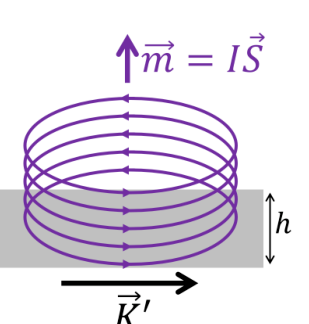
\includegraphics[width=\linewidth]{m2_bound_surface.png}
\end{column}
\end{columns}
管内 $\vct B$ 与同样 $nI$ 的真空螺线管相同，但螺线管内是有 $\vct H$、没有 $\vct M$，永磁棒内是有 $\vct M$、没有 $\vct H$。按 $\vct H$ 对应 $\vct E$，无限长样品的退磁场为零，$\vct H_{\rm in}=0$，同样得到 $\vct B_{\rm in}=\muo\vct M$。

\src{张讲义例7.3；教材例6.4；DC6，PDF24--25、例12。}
\end{frame}

\begin{frame}{螺线管中的磁介质}
\begin{columns}[T,onlytextwidth]
\begin{column}{0.66\textwidth}
无限长螺线管内充满各向同性线性介质，每单位长度 $n$ 匝，传导电流 $I$。

环路套住的是传导电流，
\[
 H_{\rm in}=nI,\qquad H_{\rm out}=0.
\]
再由本构关系，
\[
 M=\chi_m nI,\qquad
 B_{\rm in}=\mu nI=\mu_r\muo nI.
\]
顺磁质 $\chi_m>0$，磁化电流与传导电流同向，管内 $\vct B$ 比真空大。逆磁质相反。
\end{column}
\begin{column}{0.30\textwidth}
\centering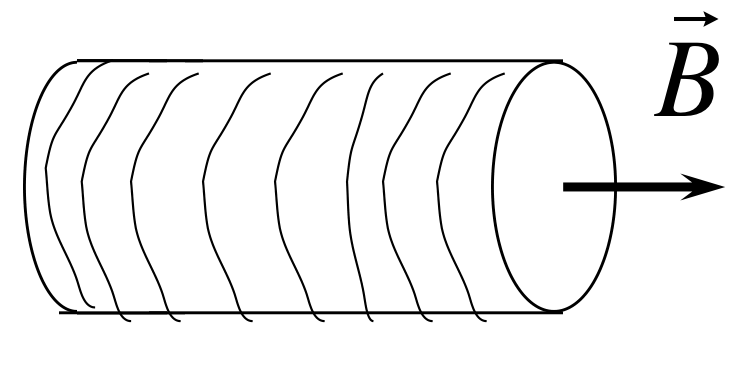
\includegraphics[width=\linewidth]{m2_filled_solenoid.png}
\end{column}
\end{columns}
\src{张讲义例7.2；教材例6.6；DC6，PDF25--27。}
\end{frame}

\begin{frame}{载流介质圆柱}
无限长圆柱半径 $R$、磁导率 $\mu$，内部均匀传导电流 $\vct J_0=J_0\vct e_z$，柱外真空。环路定理先给出 $\vct H$，它只由 $\vct J_0$ 决定。
\begin{columns}[T,onlytextwidth]
\begin{column}{0.78\textwidth}
\[
 H_\phi=\begin{cases}J_0 r/2,&r<R,\\J_0 R^2/(2r),&r>R,\end{cases}
 \qquad
 B_\phi=\begin{cases}\mu H_\phi,&r<R,\\\muo H_\phi,&r>R.\end{cases}
\]
柱内 $\vct M=\chi_m J_0 r\,\vct e_\phi/2$，因此
\[
 \vct J'=\chi_m J_0\vct e_z,\qquad
 \vct K'=-\frac{\chi_m J_0 R}{2}\vct e_z.
\]
体磁化电流与面磁化电流之和为零。柱外 $\vct B$ 与真空中同一传导电流的场相同。
\end{column}
\begin{column}{0.18\textwidth}
\centering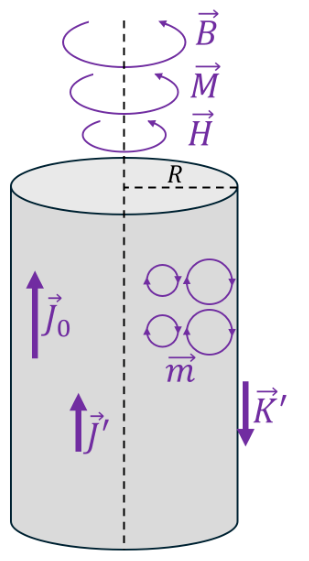
\includegraphics[height=130pt]{m2_magnetic_cylinder.png}
\end{column}
\end{columns}
柱面没有传导面电流，$H_\phi$ 连续。$\mu\neq\muo$ 时 $B_\phi$ 跃变。$\chi_m=\mu_r-1$，逆磁质的 $\vct J'$ 与 $\vct J_0$ 反向。
\src{张讲义例7.1，式(7.23)--(7.27)；DC6，PDF28--29。}
\end{frame}

\begin{frame}{磁化球}
均匀磁化球的 $\vct M$ 是常矢量，球外真空，没有传导电流。按 $\vct H$ 对应 $\vct E$、$\muo\vct M$ 对应 $\vct P$，均匀极化球的退极化场换成
\[
 \vct H_{\rm in}=-\frac{\vct M}{3},\qquad
 \vct B_{\rm in}=\frac{2\muo}{3}\vct M.
\]
总磁矩 $\vct m=(4\pi R^3/3)\vct M$。球外是这个磁矩的偶极场。

$\vct H_{\rm in}$ 与 $\vct M$ 反向，叫做退磁场。长圆柱里退磁场为零，球里是 $-\vct M/3$，很扁的盘接近 $-\vct M$。代换时用 $\vct M$ 对应 $\vct P/\epso$，分母里不再写 $\muo$。写成 $-\muo\vct M/3$ 就多了一个 $\muo$。
\src{张讲义习题7.2；教材第6.8节。球外偶极场与圆电流远场同一形式。}
\end{frame}

\begin{frame}{磁介质球}
线性介质球放在均匀外场 $\vct H_0$ 中，球外为真空，$\vct B_0=\muo\vct H_0$。静电场中介质球的内场是
\[
 \vct E_{\rm in}=\frac{3\epso}{\varepsilon+2\epso}\vct E_0.
\]
按 $\vct H$ 对应 $\vct E$、$\muo$ 对应 $\epso$、$\mu$ 对应 $\varepsilon$，
\[
 \boxed{\vct H_{\rm in}=\frac{3\muo}{\mu+2\muo}\vct H_0},
 \qquad
 \vct B_{\rm in}=\frac{3\mu}{\mu+2\muo}\vct B_0.
\]
\[
 \vct M=\frac{3(\mu-\muo)}{\mu+2\muo}\vct H_0.
\]
先得到 $\vct H_{\rm in}$，再乘 $\mu$ 得到 $\vct B_{\rm in}$。分子上是 $3\mu$，也就是 $3\mu_r\vct B_0/(\mu_r+2)$。

$\mu=\muo$ 时球不磁化。$\mu$ 很大时球内 $\vct H$ 趋于零，磁感应线被吸进球内。
\src{教材例6.13，由例2.8按 $\vct H$ 对应 $\vct E$ 代换；张讲义习题7.3。}
\end{frame}

\begin{frame}{顺磁质与铁磁质}
\begin{columns}[T,onlytextwidth]
\begin{column}{0.66\textwidth}
逆磁质的分子没有固有磁矩，外场感应出的磁矩与外场反向，$\chi_m<0$，$\mu_r<1$，数值通常比 $1$ 只小百万分之一量级。

顺磁质有固有磁矩，外场使它们趋向与外场平行，热运动把取向打乱，$\chi_m>0$ 但仍然远小于 $1$。

铁磁质里磁矩成畴。外场使畴壁移动、磁矩转向，可以达到饱和，去掉外场后还留下剩磁。$\vct B$ 与 $\vct H$ 不是单值的线性关系，还取决于磁化历史。回线包围的面积对应一个循环里损耗的能量。矫顽力大的是硬磁，用来做永磁体；矫顽力小的是软磁，用来做变压器铁芯。
\end{column}
\begin{column}{0.30\textwidth}
\centering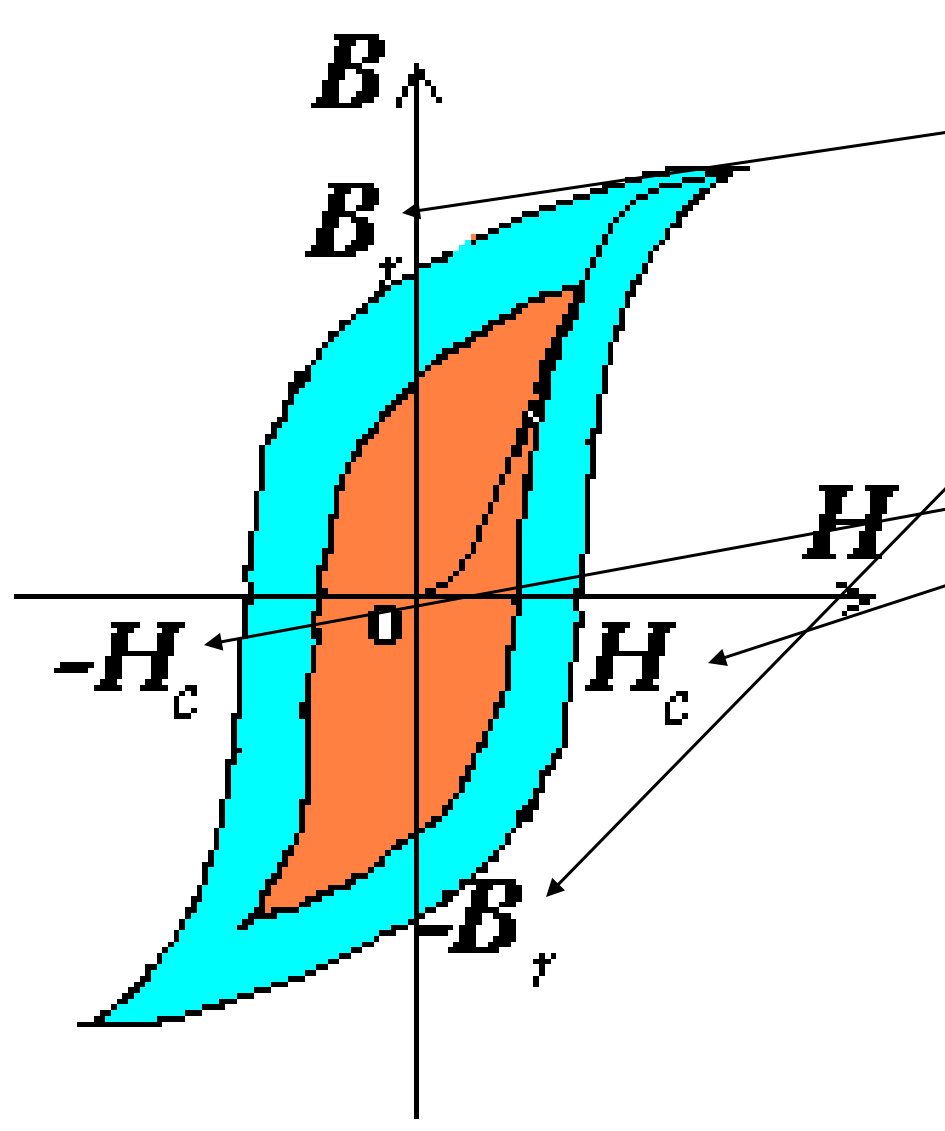
\includegraphics[height=175pt]{m2_hysteresis.png}
\end{column}
\end{columns}
\src{张讲义，PDF145--147、153；DC6，PDF15--20、55--62。}
\end{frame}

\begin{frame}{磁路}
磁感应线集中在铁芯里形成的通路叫做磁路。$\mu\gg\muo$ 时，漏到空气中的磁通可以忽略。沿一条磁路，磁通 $\Phi_B=BS$ 近似不变。

对闭合磁路，安培环路定理写成
\[
 NI=\oint\vct H\cdot\dd\vct l=\Phi_B\sum_i R_{m,i},
 \qquad
 R_m=\frac{l}{\mu S}.
\]
$NI$ 叫磁动势，$R_m$ 叫磁阻。磁动势等于各段磁势降 $\Phi_B R_m$ 之和。截面和材料分段均匀时，第 $i$ 段用该段的 $l_i$、$\mu_i$、$S_i$。

这是和直流电路的对应：磁通对电流，磁动势对电动势，磁阻 $l/(\mu S)$ 对电阻 $l/(\sigma S)$。这里 $\vct H$ 对电路中的电场，$\vct B$ 对电流密度，$\mu$ 对电导率。

介质球用的是另一套：$\vct H$ 对 $\vct E$，$\vct B$ 对 $\vct D$，$\mu$ 对 $\varepsilon$。磁路里 $\vct B$ 对的是电流密度，磁阻用 $l/(\mu S)$。

铁芯的 $\mu$ 要远大于 $\muo$，气隙要窄，否则漏磁不能忽略。软磁近似把 $\mu$ 当成常数。
\src{教材第6.7节，式(6.7.11)、(6.7.12)；DC6，第6.4节。}
\end{frame}

\begin{frame}{带气隙的磁路}
铁芯长度 $l$、截面积 $S$、磁导率 $\mu$，线圈 $N$ 匝、电流 $I$。气隙长度 $d$，气隙窄，截面仍按 $S$ 算，漏磁忽略。
\[
 NI=\Phi_B\left(\frac{l}{\mu S}+\frac{d}{\muo S}\right).
\]
没有气隙时
\[
 \Phi_B=\frac{\mu S\,NI}{l}.
\]
磁通减到这个值的一半时，
\[
 d=\frac{\muo}{\mu}\,l.
\]
铁芯磁阻是 $l/(\mu S)$，气隙磁阻是 $d/(\muo S)$。$\mu/\muo$ 常在 $10^3$ 以上，气隙只有铁芯长度的千分之一，两段磁阻就一样大，磁通主要由这段短气隙决定。

气隙里 $H$ 大约是铁芯里的 $\mu/\muo$ 倍，$\vct B$ 则两侧接近。
\src{教材第6.7.2节，图6.24及日光灯镇流器一例；DC6，例13。}
\end{frame}

\section{电磁感应与电磁波}
\gdef\coursepart{电磁感应与电磁波}

\begin{frame}{电磁感应与电磁波}
电磁感应是磁通变化时回路中产生电动势的现象；电磁波是变化的电场与磁场相互激发、在空间中传播的波。
基本性质：法拉第电磁感应定律（动生与感生），位移电流（变化的电场进入安培环路）。与两个高斯定律合在一起，写成麦克斯韦方程组。

几类电磁感应与电磁波问题的一般方法：\\
（1）电动势：动生用 $\vct v\times\vct B$，感生用法拉第定律\\
（2）电路问题：自感、互感、磁场能量与 $RL$ 暂态\\
（3）位移电流补进安培环路，写成麦克斯韦方程组，和边值关系一并求解\\
（4）能动量：坡印廷矢量，动量和角动量守恒\\
（5）电磁波：波动方程与平面波，界面上求反射和折射
\src{张讲义第八、九章；DC7、DC8、DC10；缪讲义电磁感应、位移电流与电磁波。}
\end{frame}

\begin{frame}{动生电动势}
导体相对磁场运动时，其中的载流子受到洛伦兹力。单位正电荷受到的力是 $\vct v\times\vct B$，方向和大小都与静电场力 $\vct E$ 相同，所以把它看成等效电场。
\[
 \mathcal{E}=\int(\vct v\times\vct B)\cdot\dd\vct l.
\]
$\vct v$ 是导体上该点相对磁场的速度，$\dd\vct l$ 沿导线从一端指向另一端。$\vct v$ 与 $\vct B$ 平行的一段，贡献为零。

开路时，电荷移到两端，静电场与 $\vct v\times\vct B$ 平衡，两端电势差等于这个电动势。闭合时，电流等于电动势除以回路电阻。

直杆长 $\ell$，在均匀磁场里平动，并且 $\vct v$、$\vct B$、杆三者两两垂直时，$\mathcal{E}=B\ell v$。速度或磁场沿杆不均匀时，必须沿杆积分。
\src{张讲义第8.1--8.2节，式(8.7)--(8.9)；DC7，动生电动势。}
\end{frame}

\begin{frame}{感生电动势}
磁场随时间变化时，空间中产生感生电场。它沿闭合曲线的积分一般不为零：
\[
 \oint_C\vct E\cdot\dd\vct l
 =-\frac{\dd\Phi_B}{\dd t}
 =-\int_S\frac{\partial\vct B}{\partial t}\cdot\dd\vct S.
\]
感生电场不是保守场，有旋度，不能写成某个电势的梯度。

回路正向和曲面法向成右手关系。负号表示感应电流自己产生的磁通，阻碍引起感应的那个磁通变化。

一般会利用对称性把 $E$ 从积分号里提出来计算
\src{张讲义第8.2节，式(8.13)、(8.23)；DC7，感生电场。}
\end{frame}

\begin{frame}{电动势}
合并动生和感生两种电动势，有：
\[
 \boxed{\mathcal{E}
 =\oint_C(\vct E+\vct v\times\vct B)\cdot\dd\vct l
 =-\frac{\dd\Phi_B}{\dd t}}.
\]
$\vct E$ 是感生电场，$\vct v\times\vct B$ 是运动导体里的等效电场。右边是回路所围磁通的变化率。

\src{张讲义式(8.9)、(8.13)、(8.23)；DC7。}
\end{frame}

\begin{frame}{滑动导体杆}
\begin{columns}[T,onlytextwidth]
\begin{column}{0.34\textwidth}
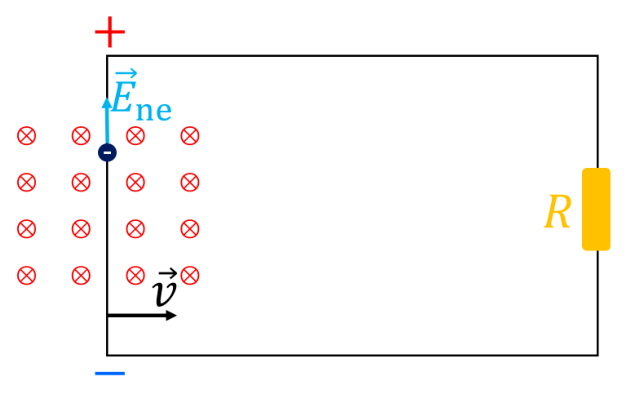
\includegraphics[width=\linewidth]{m3_sliding_rod.png}

杆长 $\ell$，速度 $v$ 向右。磁场垂直纸面向内，回路电阻为 $R$。
\end{column}
\begin{column}{0.62\textwidth}
等效电场 $\vct v\times\vct B$ 向上，
\[
 \mathcal{E}=B\ell v.
\]
上端电势高，电流沿顺时针方向。
\[
 I=\frac{B\ell v}{R},\qquad
 F_B=\frac{B^2\ell^2}{R}v.
\]
磁力向左，阻碍杆向右运动。匀速时外力向右，外力的功率等于焦耳热：
\[
 F_{\rm ext}v=\mathcal{E}I=I^2R.
\]
\end{column}
\end{columns}
磁力始终垂直于载流子的总速度，不对载流子做功。焦耳热来自外力。撤去外力后
\[
 m\dot v=-\frac{B^2\ell^2}{R}v,\qquad
 v=v_0\e^{-t/\tau},\qquad
 \tau=\frac{mR}{B^2\ell^2}.
\]
这里忽略了自感，电流随速度立刻变化。
\src{张讲义发电机原理；DC7；缪讲义磁阻尼。}
\end{frame}

\begin{frame}{圆形磁场}
\begin{columns}[T,onlytextwidth]
\begin{column}{0.28\textwidth}
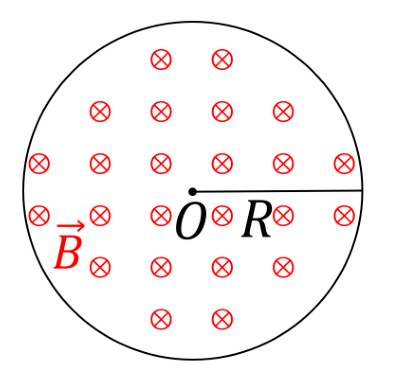
\includegraphics[width=\linewidth]{m3_finite_B.png}

磁场局限在半径 $R$ 的圆柱内，方向垂直纸面。
\end{column}
\begin{column}{0.68\textwidth}
$B_z(t)$ 以向外为正，感生电场 $E_\varphi$ 以逆时针为正。$r<R$ 时，回路围住的磁通是 $\pi r^2B_z$，
\[
 E_\varphi=-\frac{r}{2}\dot B_z.
\]
$r>R$ 时，磁通只来自半径 $R$ 以内，
\[
 E_\varphi=-\frac{R^2}{2r}\dot B_z.
\]
\end{column}
\end{columns}
$E_\varphi$ 在 $r=R$ 连续。区内随 $r$ 增大，区外按 $1/r$ 减小。区外 $B=0$，环路围住的磁通仍在变化，所以仍有感生电场。$\dot B_z>0$ 时电场沿顺时针方向。
\src{张讲义例8.3；DC7例3。}
\end{frame}

\begin{frame}{涡流}
导体盘半径 $a$、厚度 $\delta$、电导率 $\sigma$。磁场只在 $r\le R$ 内不为零，且 $R<a$，那里 $B_z=B_0(t)$。忽略涡流对这个外加磁场的反作用。

感生电场就是圆形磁区的结果，$\vct J=\sigma E_\varphi\vct e_\varphi$。焦耳热功率密度为 $\sigma E_\varphi^2$。薄环体积 $2\pi r\delta\,\dd r$，分内外两段积分：
\[
 \begin{aligned}
 P&=2\pi\delta\sigma\dot B_0^{\,2}
 \left(\int_0^R\frac{r^3}{4}\,\dd r
 +\int_R^a\frac{R^4}{4r}\,\dd r\right)\\
 &=\boxed{\dfrac{\pi\delta\sigma R^4}{8}\dot B_0^{\,2}
 \left(1+4\ln\frac{a}{R}\right)}.
 \end{aligned}
\]
括号里第一项来自磁区内部，对数项来自外部环形导体。只改变外半径 $a$ 时，变的是第二项。

这个算法要求外加 $B_0(t)$ 已知。涡流很强、足以改变磁通时，要先把反作用算进 $B$。
\src{期中复习笔记题7.6；缪讲义6.2；DC7涡流。}
\end{frame}

\begin{frame}{旋转圆盘}
\begin{columns}[T,onlytextwidth]
\begin{column}{0.30\textwidth}
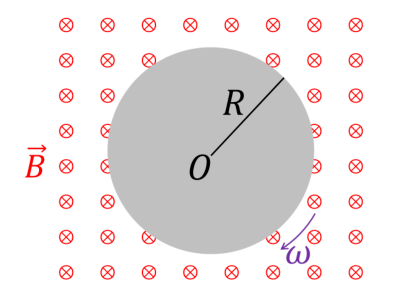
\includegraphics[width=\linewidth]{m3_rotating_disk.png}

半径 $R$ 的导体盘绕轴转动，均匀磁场垂直盘面。图中 $\vct\omega$ 与 $\vct B$ 同向。
\end{column}
\begin{column}{0.66\textwidth}
距轴 $s$ 处速度为 $\omega s$，正电荷受力沿径向向外。中心到边缘
\[
 \mathcal{E}
 =\int_0^R\omega s B\,\dd s
 =\frac12 B\omega R^2.
\]
开路达到平衡时，$\vct E+\vct v\times\vct B=0$，边缘电势比中心高 $\dfrac12 B\omega R^2$。电刷接通中心和边缘后，回路里才有持续电流。
\end{column}
\end{columns}
盘的面积不变，总磁通也不变。中心到边缘是开路，电动势沿半径对 $\vct v\times\vct B$ 积分。
\src{张讲义例8.1；DC7动生电动势。}
\end{frame}

\begin{frame}{电磁刹车}
\begin{columns}[T,onlytextwidth]
\begin{column}{0.30\textwidth}
\centering
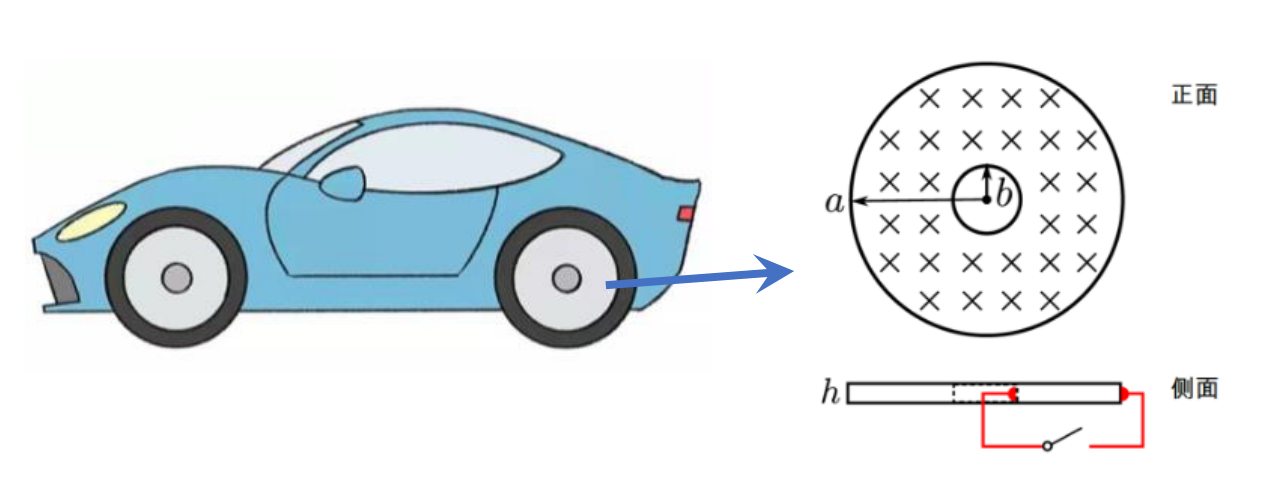
\includegraphics[width=\linewidth]{sample_brake.png}
\end{column}
\begin{column}{0.66\textwidth}
车轮半径 $r$，盘的内外半径 $b$、$a$，厚度 $h$，电阻率 $\rho$，磁场 $B$ 垂直盘面。纯滚动时 $\omega=v/r$。忽略外接电阻、自感和轮子转动惯量。径向薄环串联，截面积是 $2\pi sh$：
\[
 R=\frac{\rho}{2\pi h}\ln\frac{a}{b},\qquad
 \mathcal{E}=\frac{B(a^2-b^2)}{2r}\,v.
\]
$\vct\omega$ 与 $\vct B$ 同向时外缘电势高。功率 $P=\mathcal{E}^2/R=kv^2$，
\[
 k=\frac{B^2(a^2-b^2)^2}{4r^2R}.
\]
$h$ 越大，电阻越小。
\end{column}
\end{columns}
\src{往年期中考试样卷第4题(1)(2)(3)。}
\end{frame}

\begin{frame}{刹车距离}
题目规定，损失的动能都变成焦耳热，车辆质量为 $M$：
\[
 -\frac{\dd}{\dd t}\!\left(\frac12 Mv^2\right)=kv^2,
 \qquad M\dot v=-kv.
\]
\[
 v=v_0\e^{-t/\tau},\qquad \tau=\frac{M}{k},
 \qquad s=\tau(v_0-v_1).
\]
题设 $r=0.25\unit{m}$，$a=0.20\unit{m}$，$b=0.05\unit{m}$，$h=0.02\unit{m}$，$\rho=10^{-8}\,\Omega\cdot\mathrm{m}$，$B=0.1\unit{T}$，$M=2000\unit{kg}$。
\[
 R=1.103\times10^{-7}\,\Omega,\qquad
 k=509.9\,\mathrm{kg\,s^{-1}},\qquad
 \tau=3.922\unit{s}.
\]
从 $100$ 降到 $10$，单位是 $\mathrm{km\cdot h^{-1}}$，
\[
 t=\tau\ln 10=9.03\unit{s},\qquad
 s=\boxed{98.1\unit{m}}.
\]
速度越低，制动力越弱。这个模型里速度降到零要无限长时间，滑行距离趋近 $\tau v_0$。
\src{样卷第4题(4)(5)。$s=\tau(v_0-v_1)$ 中速度用 $\mathrm{m\,s^{-1}}$。}
\end{frame}

\begin{frame}{自感}
线圈中的电流变化时，它自己的磁通也变化，由此产生的电动势叫做自感电动势。我们可以定义磁通匝链数$Psi$等于各匝磁通之和，且有：
\[
 \Psi=LI,\qquad
 \mathcal{E}=-L\frac{\dd I}{\dd t}.
\]
$L$ 叫做自感系数。它由线圈的形状、匝数和介质决定，与电流无关。有铁磁质时 $B$ 与 $I$ 不成正比，$L$ 还随电流变化，$L$一般很难计算 。

计算时先由电流求 $\vct B$，再对每一匝积分磁通，相加得到 $\Psi$，然后 $L=\Psi/I$。

长直螺线管长 $l$，截面积 $S$，总匝数 $N$，管内 $B=\muo NI/l$，管外磁场忽略，
\[
 \boxed{L=\muo\frac{N^2S}{l}}.
\]
$l$ 不远大于半径时，两端漏磁，实际自感比这个值小。单位长度的自感是 $\muo n^2S$，$n=N/l$。
\src{张讲义第8.3节，式(8.46)及长直螺线管例题；DC7。}
\end{frame}

\begin{frame}{互感}
线圈 1 的电流在线圈 2 中产生磁链。线性介质、相对位置不变时
\[
 \Psi_{21}=M_{21}I_1,\qquad
 \mathcal{E}_2=-M_{21}\frac{\dd I_1}{\dd t}.
\]
$M_{21}$ 叫做互感系数。没有铁磁质时它与电流无关，并且
\[
 M_{12}=M_{21}=M.
\]
$M$ 的正负看两个回路的正向：正向取得一致时 $M>0$。只把一个回路的正向反过来，$M$ 变号。

两个空气芯长螺线管共轴、等长 $l$，截面积 $S_1<S_2$，匝数 $N_1$、$N_2$，$l$ 远大于半径。内管的磁场 $B_1=\muo N_1I_1/l$ 只分布在 $S_1$ 上，外管每一匝围住的有效面积仍是 $S_1$，
\[
 \boxed{M=\muo\frac{N_1N_2S_1}{l}}.
\]
改由外管的电流计算，内管处 $B_2=\muo N_2I_2/l$，每匝内管的面积还是 $S_1$，得到同一个 $M$。漏磁忽略时，$M/\sqrt{L_1L_2}=\sqrt{S_1/S_2}$。
\src{张讲义例8.5；DC7长螺线管的自感与互感。}
\end{frame}

\begin{frame}{磁场能量}
建立电流时，电源要克服自感电动势做功。线性介质里，一个线圈储存的磁场能量是
\[
 W_m=\int_0^I Li\,\dd i=\frac12 LI^2.
\]
两个线圈还要加上互感的功。$M$ 按前面的正向约定，
\[
 W_m=\frac12 L_1I_1^2+\frac12 L_2I_2^2+MI_1I_2.
\]
$M$ 可以为负，但整个 $W_m$ 不能为负，因此 $|M|\le\sqrt{L_1L_2}$。

同一能量也可以对场积分。各向同性线性介质中，能量密度是
\[
 w_m=\frac12\vct B\cdot\vct H=\frac{B^2}{2\mu}.
\]
对全空间积分，结果与电路公式一致。电流不好归成一个 $L$ 时，先积 $B^2/(2\mu)$，再由 $W_m=\dfrac12 LI^2$ 反解 $L$。铁磁质的磁化与历史有关，不能再用这个式子。
\src{张讲义第8.4节，式(8.55)、(8.73)；DC8。}
\end{frame}

\begin{frame}{RL电路}
\begin{columns}[T,onlytextwidth]
\begin{column}{0.24\textwidth}
\centering
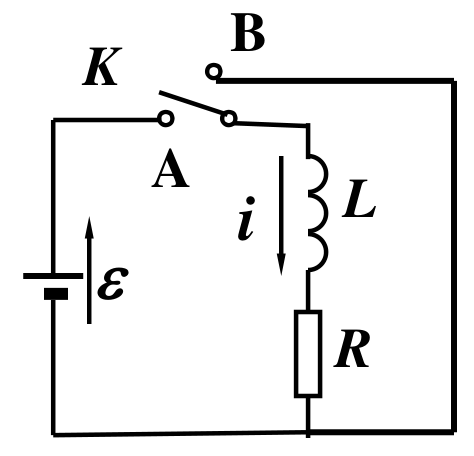
\includegraphics[width=\linewidth]{m3_RL.png}
\end{column}
\begin{column}{0.72\textwidth}
线性电感与电阻串联，时间常数 $\tau=L/R$，$R$ 含线圈电阻。电流不能突变。
\[
 L\frac{\dd i}{\dd t}+Ri=\mathcal{E}_0,\qquad
 i=\frac{\mathcal{E}_0}{R}\bigl(1-\e^{-t/\tau}\bigr).
\]
接通前电流为零。电源功率分成电阻发热和磁场能量的增加：
\[
 \mathcal{E}_0 i=Ri^2+\frac{\dd}{\dd t}\!\left(\frac12 Li^2\right).
\]
\end{column}
\end{columns}
开关改接到电阻上，初电流为 $I_0$ 时 $i=I_0\e^{-t/\tau}$，放出的热量等于 $\dfrac12 LI_0^2$。直流稳定后 $\dd i/\dd t=0$，理想电感两端电压为零。
\src{DC7，RL暂态；张讲义自感电动势与磁能。}
\end{frame}

\begin{frame}{位移电流}
稳恒时 $\nabla\times\vct H=\vct J_f$。两边取散度，得到 $\nabla\cdot\vct J_f=0$。电荷若在某处积累，连续性方程是
\[
 \nabla\cdot\vct J_f+\frac{\partial\rho_f}{\partial t}=0,
\]
与上面的结论矛盾。又因为 $\nabla\cdot\vct D=\rho_f$，所以可以引入位移电流
\[
 \nabla\cdot\!\left(\vct J_f+\frac{\partial\vct D}{\partial t}\right)=0.
\]
安培环路改成
\[
 \boxed{\nabla\times\vct H
 =\vct J_f+\frac{\partial\vct D}{\partial t}},
 \qquad
 \vct J_d\equiv\frac{\partial\vct D}{\partial t}.
\]
$\vct J_d$ 叫做位移电流密度。通过一个曲面的位移电流是 $I_d=\int\vct J_d\cdot\dd\vct S$。真空中 $\vct J_d=\epso\partial\vct E/\partial t$。

它描述变化的电场，不是电荷在导线里流动。电容器充电时，导线里有传导电流，极板之间没有；不写 $\vct J_d$，同一个环路会因所选曲面不同而得到不同的环流。补上以后，穿过导线的传导电流和穿过极板间隙的位移电流相等。
\src{张讲义第9.1节，式(9.2)--(9.5)；DC10；缪讲义8.1。}
\end{frame}

\begin{frame}{e.g,4.2费曼圆形电容器}
圆形平行板半径 $a$，间距 $d$，且 $d\ll a$，忽略边缘效应。两端接交变电压 $V=V_0\cos\omega t$。板间电场沿轴线。尺寸远小于波长时，按 $(\omega r/c)^2$ 逐级计算。

零阶先不计磁场。电场由电压决定，板间近似均匀，
\[
 E_z^{(0)}=\frac{V_0}{d}\cos\omega t.
\]
这个电场的变化率就是位移电流。$r<a$ 时，半径 $r$ 的环路围住 $\pi r^2$ 上的位移电流，
\[
 B_\varphi^{(1)}
 =-\frac{\muo\epso\omega r}{2}\frac{V_0}{d}\sin\omega t
 =-\frac{\omega r}{2c^2}\frac{V_0}{d}\sin\omega t.
\]
$r>a$ 时，位移电流只通过半径 $a$ 的圆面，$B_\varphi$ 按 $a^2/r$ 减小。

零阶电场是静电场的结果。磁场比它多一个因子 $\omega r/c^2$，是下一级小量。下面只用板间的 $B_\varphi^{(1)}$ 去修正电场。
\src{费曼物理学讲义第二卷，交变电压下的圆形电容器。}
\end{frame}

\begin{frame}{e.g,4.3费曼圆形电容器}
包含轴线的小矩形回路上，磁通来自 $B_\varphi$，因此 $\partial E_z/\partial r=\partial B_\varphi/\partial t$。代入上一级磁场，并把轴上的修正取为零：
\[
 \begin{aligned}
 E_z^{(2)}
 &=-\frac14\left(\frac{\omega r}{c}\right)^2\frac{V_0}{d}\cos\omega t,\\
 E_z^{(4)}
 &=\frac{1}{64}\left(\frac{\omega r}{c}\right)^4\frac{V_0}{d}\cos\omega t.
 \end{aligned}
\]
二阶电场的位移电流再产生磁场，这个磁场再用法拉第定律给出四阶电场。每一级都比上一级多 $(\omega r/c)^2$。$a$ 远小于波长时，二阶已经很小，板间可以用均匀的零阶电场。

\src{费曼物理学讲义第二卷，圆形电容器的逐级近似。这里不把级数收成贝塞尔函数。}
\end{frame}

\begin{frame}{麦克斯韦方程组}
自由电荷密度为 $\rho_f$，传导电流密度为 $\vct J_f$：
\begin{columns}[T,onlytextwidth]
\begin{column}{0.58\textwidth}
\textbf{积分形式}
\[
 \begin{aligned}
 \oiint\vct D\cdot\dd\vct S&=Q_{f,{\rm in}}\\
 \oiint\vct B\cdot\dd\vct S&=0\\
 \oint\vct E\cdot\dd\vct l
 &=-\frac{\dd}{\dd t}\int\vct B\cdot\dd\vct S\\
 \oint\vct H\cdot\dd\vct l
 &=I_{f,{\rm in}}+\frac{\dd}{\dd t}\int\vct D\cdot\dd\vct S
 \end{aligned}
\]
\end{column}
\begin{column}{0.40\textwidth}
\textbf{微分形式}
\[
 \begin{aligned}
 \nabla\cdot\vct D&=\rho_f\\
 \nabla\cdot\vct B&=0\\
 \nabla\times\vct E&=-\partial_t\vct B\\
 \nabla\times\vct H
 &=\vct J_f+\partial_t\vct D
 \end{aligned}
\]
\end{column}
\end{columns}
介质的本构关系不假定线性：
\[
 \vct D=\epso\vct E+\vct P,\qquad
 \vct B=\muo(\vct H+\vct M).
\]
$\vct P$、$\vct M$ 由介质和它的历史决定，不必与场成正比。
\src{张讲义第9.2节；DC10。$\vct D$、$\vct B$ 的定义不要求线性介质。}
\end{frame}

\begin{frame}{边值关系}
界面两侧分别记为 1 和 2，$\hat{\vct n}$ 从 1 指向 2。界面上自由面电荷为 $\sigma_f$，自由面电流为 $\vct K_f$。场在界面附近保持有限时，
\[
 \begin{aligned}
 \hat{\vct n}\cdot(\vct D_2-\vct D_1)&=\sigma_f,\\
 \hat{\vct n}\cdot(\vct B_2-\vct B_1)&=0,\\
 \hat{\vct n}\times(\vct E_2-\vct E_1)&=0,\\
 \hat{\vct n}\times(\vct H_2-\vct H_1)&=\vct K_f.
 \end{aligned}
\]
法向的 $\vct D$、$\vct B$ 来自高斯型的两个方程，用扁柱面。切向的 $\vct E$、$\vct H$ 来自环路型的两个方程，用跨在界面上的窄矩形。时间变化的通量在扁柱和窄矩形上是高阶小量，所以这四式对静场和时变场都用。

自由面电荷使法向 $\vct D$ 跳变，自由面电流使切向 $\vct H$ 跳变。没有自由面电荷和自由面电流时，法向 $\vct B$、$\vct D$ 连续，切向 $\vct E$、$\vct H$ 连续。电磁波在介质表面的反射和折射就用这一组。
\src{张讲义界面条件与第9.2节；DC10。}
\end{frame}

\begin{frame}{电磁场的能量}
电动力学里，场对介质做的元功密度是
\[
 \delta w=\vct E\cdot\delta\vct D+\vct H\cdot\delta\vct B.
\]
这里不要求 $\vct D$、$\vct B$ 与 $\vct E$、$\vct H$ 成正比。

线性、无色散、无磁滞时，沿场从零建立的过程积分，得到能量密度
\[
 u=\frac12\vct E\cdot\vct D+\frac12\vct B\cdot\vct H
 =\frac12\varepsilon E^2+\frac12\mu H^2.
\]
\src{张讲义第9.4节，式(9.77)--(9.79)。元功 $\vct E\cdot\delta\vct D+\vct H\cdot\delta\vct B$ 不依赖线性假设。}
\end{frame}

\begin{frame}{坡印廷矢量}
由 $\nabla\times\vct E=-\partial\vct B/\partial t$ 和 $\nabla\times\vct H=\vct J_f+\partial\vct D/\partial t$，在线性无色散介质中得到
\[
 \boxed{\frac{\partial u}{\partial t}+\nabla\cdot\vct S
 =-\vct J_f\cdot\vct E},
 \qquad
 \boxed{\vct S=\vct E\times\vct H}.
\]
$\vct S$ 叫做坡印廷矢量，方向是电磁能量流动的方向，大小是单位时间通过垂直于该方向的单位面积的能量。

对固定体积积分，边界外法向为 $\dd\vct A$，
\[
 -\oiint\vct S\cdot\dd\vct A
 =\frac{\dd}{\dd t}\int u\,\dd V
 +\int\vct J_f\cdot\vct E\,\dd V.
\]
左边是单位时间流入这个体积的电磁能量。右边第一项是场能的增加，第二项是场对电流做功的功率，相当于焦耳热。
稳恒时场能不变，流入的功率等于焦耳热。没有电流时，流入的功率等于场能的增加率。
\src{张讲义第9.4节，式(9.84)--(9.92)；DC10。}
\end{frame}

\begin{frame}{电阻中的能流}
\begin{columns}[T,onlytextwidth]
\begin{column}{0.68\textwidth}
圆柱电阻长 $L$、半径 $a$，两端电压 $U$，稳恒电流 $I$ 沿 $+z$。柱内
\[
 E_z=\frac{U}{L},\qquad
 H_\varphi(a)=\frac{I}{2\pi a}.
\]
侧面的坡印廷矢量指向轴，
\[
 \vct S(a)=-\frac{UI}{2\pi a L}\vct e_r.
\]
从整个侧面流入的功率是
\[
 P=-\int\vct S\cdot\dd\vct A=UI.
\]
\end{column}
\begin{column}{0.28\textwidth}
\centering
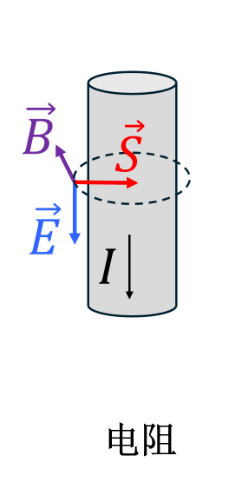
\includegraphics[height=4.2cm]{m4_resistor_energy_flow.png}
\end{column}
\end{columns}
电能从侧面进入导体，变成焦耳热。电场和磁场都可以不随时间变化。$H_\varphi$ 用柱面外缘的安培环路；电流均匀时，内部任一圆柱侧面流入的功率等于该圆柱内的焦耳热。
\src{张讲义坡印廷矢量的电阻例子；DC10；教材习题10.7。}
\end{frame}

\begin{frame}{电磁场的动量}
真空中，电磁场的动量密度是
\[
 \boxed{\vct g=\epso\vct E\times\vct B=\frac{\vct S}{c^2}}.
\]
$\vct S$ 沿能量传播的方向，动量也沿这个方向。一段真空中的波若携带能量 $U$，它的动量大小就是 $U/c$。

波垂直射到不透明的表面上，入射强度为 $I$，照射面积为 $A$。单位时间入射的能量是 $IA$，带来的动量是 $IA/c$。全部被吸收时，交给表面的动量就是这些，压强为 $I/c$。全部被垂直反射时，反射波带走相反的动量，表面得到的动量是入射的两倍，压强为 $2I/c$。反射率是 $R$、其余都被吸收时，压强是 $(1+R)I/c$。

介质里动量密度有不止一种写法。一般考试也不会考（除非出卷人相对恶意）
\src{张讲义第9.4节；DC10；教材第10章。}
\end{frame}

\begin{frame}{光压}
光强为 $I$，光线与平面法线的夹角为 $\theta$，镜面的实际面积为 $A$，镜面不透光。单位时间射到镜面上的能量是 $IA\cos\theta$，因为光束的横截面积是 $A\cos\theta$。

动量沿光线方向。全反射时，法向动量的改变还要再乘一个 $\cos\theta$，法向压强是
\[
 \boxed{p_n=\frac{2I}{c}\cos^2\theta}.
\]
吸收的份额为 $\alpha$，其余仍按镜面反射时，
\[
 p_n=\frac{(2-\alpha)I}{c}\cos^2\theta.
\]
被吸收的那一部分动量沿原来的光线，所以还有切向力。单位面积上的切向力是 $\alpha I\sin\theta\cos\theta/c$。

\src{期中复习笔记题10.9；教材习题10.9；张讲义光压。}
\end{frame}

\begin{frame}{电磁场的角动量}
相对于原点，真空中电磁场的角动量密度和总角动量是
\[
 \vct\ell=\vct r\times\vct g,
 \qquad
 \vct L=\int\vct r\times(\epso\vct E\times\vct B)\,\dd V.
\]
$\vct g$ 沿方位角、$\vct r$ 沿径向时，$\vct\ell$ 沿轴线。径向电场和轴向磁场叠在一起，就是这种情形。

没有外力矩时，机械角动量与场的角动量之和守恒。外力矩的冲量等于两者之和的增加。

积分范围要包括电场和磁场同时不为零的全部区域。带电圆柱面的磁场常常在柱内，电场常常在柱外，角动量就在柱面外面。只对柱面内部积分，结果可以是零。
\src{DC10；教材电磁场的动量与角动量。介质中的动量不采用 $\vct S/c^2$。}
\end{frame}

\begin{frame}{e.g.5带电圆柱面加速}
两个共轴无限长圆柱面，半径 $a<b$。内柱单位长度电荷 $+\lambda$，外柱单位长度电荷 $-\lambda$。外力使两层以同一个角速度 $\omega(t)$ 绕轴线加速，$\omega$ 沿 $+z$。下面先不计圆柱面自己的转动惯量，外力矩只用来改变电磁场。

电荷随柱面转动，形成沿方位角的面电流
\[
 K_a=\frac{\lambda\omega}{2\pi},\qquad
 K_b=-\frac{\lambda\omega}{2\pi}.
\]
每一层都相当于一个螺线管，磁场只在该层以内。两层叠加：
\[
 B_z=
 \begin{cases}
 0,&r<a,\\
 -\muo\lambda\omega/(2\pi),&a<r<b,\\
 0,&r>b.
 \end{cases}
\]
静电场只在两层之间，$E_r=\lambda/(2\pi\epso r)$。内柱里面和外柱外面，静电场都是零。

因此 $\vct E$ 和 $\vct B$ 只在 $a<r<b$ 同时存在。这个区域在内柱面的外面。
\src{无限长带电圆柱面的电场、等效螺线管磁场。以下三页用同一模型。}
\end{frame}

\begin{frame}{e.g.5带电圆柱面加速-力矩法}
$\omega$ 增大时，只有 $a<r<b$ 的磁通在变。环路正向与 $+z$ 成右手关系，$a<r<b$ 时
\[
 \Phi_B=B_z\,\pi(r^2-a^2)
 =-\frac{\muo\lambda\omega}{2}(r^2-a^2).
\]
\[
 E_\varphi=\frac{\muo\lambda\dot\omega\,(r^2-a^2)}{4\pi r}.
\]
内柱面 $r=a$ 上 $E_\varphi=0$，感生电场对内柱面没有力矩。外柱面
\[
 E_\varphi(b)=\frac{\muo\lambda\dot\omega\,(b^2-a^2)}{4\pi b}.
\]
外柱面单位长度电荷是 $-\lambda$，受力与 $E_\varphi$ 相反，力矩沿 $-z$，阻碍加速。单位长度上，这个力矩的大小是
\[
 \tau=\frac{\muo\lambda^2(b^2-a^2)}{4\pi}\dot\omega.
\]
忽略转动惯量时，外力矩与它平衡，方向沿 $+z$，大小就是 $\tau$。电磁力矩加在外柱面上，不加在内柱面上。
\src{法拉第定律与洛伦兹力。环路正向与 $+z$ 成右手系。}
\end{frame}

\begin{frame}{e.g.5带电圆柱面加速-角动量法}
动量密度 $\vct g=\epso\vct E\times\vct B$。$a<r<b$ 中 $\vct E$ 沿径向，$\vct B$ 沿 $-z$，所以 $\vct g$ 沿方位角。角动量密度沿 $+z$，并且与 $r$ 无关：
\[
 \ell_z=\frac{\muo\lambda^2\omega}{4\pi^2}.
\]
对 $a<r<b$ 的圆环面积积分，单位长度的角动量是
\[
 \boxed{L_z=\frac{\muo\lambda^2\omega(b^2-a^2)}{4\pi}}.
\]
$r<a$ 时电场和磁场都是零，$r>b$ 时也是零，这两处的贡献都是零。$L_z$ 全部在内柱面之外、外柱面之内。

只对内柱面内部积分，得到的角动量是零，它的变化率也是零，和外力矩 $\tau$ 对不上。对 $a<r<b$ 积分以后，
\[
 \frac{\dd L_z}{\dd t}=\tau.
\]
外力矩的冲量等于场的角动量的增加。
\src{真空动量密度 $\epso\vct E\times\vct B$。角动量必须含 $a<r<b$。}
\end{frame}

\begin{frame}{e.g.5带电圆柱面加速-能量法}
磁场只在 $a<r<b$。单位长度的磁场能量是
\[
 U=\frac{B^2}{2\muo}\,\pi(b^2-a^2)
 =\frac{\muo\lambda^2\omega^2(b^2-a^2)}{8\pi}.
\]
外力矩的功率
\[
 \tau\omega=\frac{\muo\lambda^2\omega\dot\omega\,(b^2-a^2)}{4\pi}
 =\frac{\dd U}{\dd t}.
\]
外力做的功全部变成磁场能量。静电场的能量与 $\omega$ 无关，不进入这个功率。

感生电场的力矩、场的角动量、磁场能量，给出的是同一个外力矩
\[
 \tau=\frac{\muo\lambda^2(b^2-a^2)}{4\pi}\dot\omega.
\]
圆柱面自己还有转动惯量 $I_a$、$I_b$ 时，外力矩要再加上 $(I_a+I_b)\dot\omega$。多出来的这一部分只增加机械角动量和动能，不改变上面的磁场能量和场的角动量。
\src{三种算法：感生电场的力矩、角动量守恒、磁场能量。}
\end{frame}

\begin{frame}{波动方程}
均匀、各向同性、不导电的介质，$\varepsilon$ 和 $\mu$ 都是常数，并且没有自由电荷和传导电流。麦克斯韦方程写成
\[
 \nabla\cdot\vct E=0,\qquad
 \nabla\times\vct E=-\mu\frac{\partial\vct H}{\partial t},\qquad
 \nabla\times\vct H=\varepsilon\frac{\partial\vct E}{\partial t}.
\]
对第二式取旋度，把第三式代进去，再用
\[
 \nabla\times(\nabla\times\vct E)
 =\nabla(\nabla\cdot\vct E)-\nabla^2\vct E,
\]
得到
\[
 \boxed{\nabla^2\vct E
 =\mu\varepsilon\frac{\partial^2\vct E}{\partial t^2}},
 \qquad
 v=\frac{1}{\sqrt{\mu\varepsilon}}.
\]
$\vct H$ 满足同一个方程。真空中 $c=1/\sqrt{\muo\epso}$。

推导里用了 $\nabla\cdot\vct E=0$，也没有传导电流。若 $\vct J=\sigma\vct E$，或 $\varepsilon$ 随频率变化，方程改成亥姆霍兹方程，波会衰减，波速也与频率有关。
\src{张讲义第9.3节，式(9.43)--(9.51)；DC10。}
\end{frame}

\begin{frame}{平面波}
沿 $\vct k$ 传播的单色平面波，
\[
 \vct E=\vct E_0\cos(\vct k\cdot\vct r-\omega t),
 \qquad k=\frac{\omega}{v}.
\]
代入无源的麦克斯韦方程，
\[
 \vct k\cdot\vct E=0,\qquad
 \vct k\cdot\vct B=0,\qquad
 \vct B=\frac1v\hat{\vct k}\times\vct E.
\]
\[
 \vct H=\frac1Z\hat{\vct k}\times\vct E,
 \qquad
 Z=\sqrt{\frac{\mu}{\varepsilon}}.
\]
$\vct E$、$\vct H$ 和传播方向两两垂直，三者成右手关系。无损耗介质中的行波里，$\vct E$ 和 $\vct H$ 同相，振幅满足 $E_0=ZH_0=vB_0$。

真空波阻抗 $Z_0=\sqrt{\muo/\epso}\simeq377\,\Omega$。一个周期内的平均能流沿传播方向，大小是
\[
 I=\langle S\rangle=\frac{E_0H_0}{2}=\frac{E_0^2}{2Z}.
\]
$E_0$、$H_0$ 是峰值，有效值再除以 $\sqrt2$。
\src{张讲义第9.3节，式(9.60)--(9.76)；DC10。}
\end{frame}

\begin{frame}{介质中的电磁波}
线性无损耗介质中，波速、折射率和波阻抗是
\[
 v=\frac{1}{\sqrt{\mu\varepsilon}},\qquad
 n=\frac{c}{v}=\sqrt{\varepsilon_r\mu_r},\qquad
 Z=\sqrt{\frac{\mu}{\varepsilon}}.
\]
非磁介质 $\mu_r=1$，于是 $n=\sqrt{\varepsilon_r}$，$v=c/n$，$Z=Z_0/n$。折射率越大，波越慢，波阻抗越小。

平面行波的关系仍然是 $\vct B=\hat{\vct k}\times\vct E/v$，$\vct H=\hat{\vct k}\times\vct E/Z$。电场能量密度和磁场能量密度相等，总能量密度 $u=\varepsilon E^2$，能流 $\vct S=uv\hat{\vct k}$。

\src{张讲义第9.6节；缪讲义介质中的电磁波。}
\end{frame}

\begin{frame}{界面上的电磁波}
介质界面上没有自由面电荷，也没有自由面电流。边值关系变成：法向 $\vct B$、法向 $\vct D$ 连续，切向 $\vct E$、切向 $\vct H$ 连续。

设界面是 $z=0$，入射、反射、折射三列波在界面上要每一点、每一时刻都接得上，所以三列波的频率相同，波矢的切向分量相同。由此得到三列波的波矢在同一平面内，并且
\[
 \theta_r=\theta_i,\qquad
 n_1\sin\theta_i=n_2\sin\theta_t.
\]
第一式是反射定律，第二式是折射定律。$\theta$ 都是波矢与法线的夹角。

频率相同，是因为边界条件要对所有时刻成立。切向波矢相同，是因为边界条件要对界面上所有点成立。角度关系只来自这一条，与偏振无关。振幅还要再用切向 $\vct E$、$\vct H$ 来定。
\src{张讲义第9.7节，式(9.170)--(9.176)。}
\end{frame}

\begin{frame}{菲涅尔公式}
垂直入射时，入射波和透射波的电场沿同一方向取正。反射波传播方向相反，磁场相对电场也反过来。切向电场、切向磁场连续：
\[
 E_i+E_r=E_t,\qquad
 \frac{E_i-E_r}{Z_1}=\frac{E_t}{Z_2}.
\]
\[
 \boxed{r=\frac{E_r}{E_i}=\frac{Z_2-Z_1}{Z_2+Z_1}},
 \qquad
 \boxed{t=\frac{E_t}{E_i}=\frac{2Z_2}{Z_2+Z_1}}.
\]
非磁介质 $Z=Z_0/n$，
\[
 r=\frac{n_1-n_2}{n_1+n_2},\qquad
 t=\frac{2n_1}{n_1+n_2}.
\]
平均能流 $I=E_0^2/(2Z)$。能量反射率和能量透射率是
\[
 R=r^2,\qquad
 T=\frac{Z_1}{Z_2}t^2,\qquad R+T=1.
\]
波阻抗小的一侧，同样的电场对应更大的能流，所以透射能量比带有 $Z_1/Z_2$。
\src{张讲义式(9.197)--(9.216)；缪讲义介质表面；样卷第5题(1)(2)。}
\end{frame}

\begin{frame}{斜入射}
非磁介质，电场垂直于入射面时，切向电场就是 $E$ 本身，切向磁场带有 $\cos\theta$。仍取同一电场正向，
\[
 E_i+E_r=E_t,
\]
\[
 n_1(E_i-E_r)\cos\theta_i=n_2 E_t\cos\theta_t.
\]
\[
 r_s=\frac{n_1\cos\theta_i-n_2\cos\theta_t}
 {n_1\cos\theta_i+n_2\cos\theta_t},\qquad
 t_s=\frac{2n_1\cos\theta_i}
 {n_1\cos\theta_i+n_2\cos\theta_t}.
\]
电场在入射面内时，切向电场带有 $\cos\theta$，磁场垂直于入射面：
\[
 r_p=\frac{n_2\cos\theta_i-n_1\cos\theta_t}
 {n_2\cos\theta_i+n_1\cos\theta_t},\qquad
 t_p=\frac{2n_1\cos\theta_i}
 {n_2\cos\theta_i+n_1\cos\theta_t}.
\]
垂直入射时两种偏振的能量反射率相同。$r_p$ 和 $r_s$ 差一个符号，来自反射波电场正向的取法。用同一切向坐标取正负时，垂直入射的反射系数回到 $(n_1-n_2)/(n_1+n_2)$。

能量反射率仍是 $r^2$。斜入射的能量透射率还要乘 $\cos\theta_t/\cos\theta_i$，因为折射光束的横截面积和入射光束不同。
\src{张讲义第9.7节菲涅尔公式。非磁介质，$\mu_1=\mu_2=\muo$。}
\end{frame}

\begin{frame}{垂直入射}
\begin{columns}[T,onlytextwidth]
\begin{column}{0.66\textwidth}
平面波从真空垂直射入非磁介质，折射率 $n=\sqrt{\varepsilon/\epso}$，波阻抗 $Z=Z_0/n$。由垂直入射的菲涅尔公式，
\[
 E_r=\frac{1-n}{1+n}E_i,\qquad
 E_t=\frac{2}{1+n}E_i.
\]
平均能流 $I_i=E_i^2/(2Z_0)$，$I_r=E_r^2/(2Z_0)$，$I_t=nE_t^2/(2Z_0)$。
\[
 R=\frac{(1-n)^2}{(1+n)^2},\qquad
 T=\frac{4n}{(1+n)^2},\qquad
 R+T=1.
\]
$n>1$ 时反射电场反向。相同截面上，入射功率等于反射功率与透射功率之和。
\end{column}
\begin{column}{0.30\textwidth}
\centering
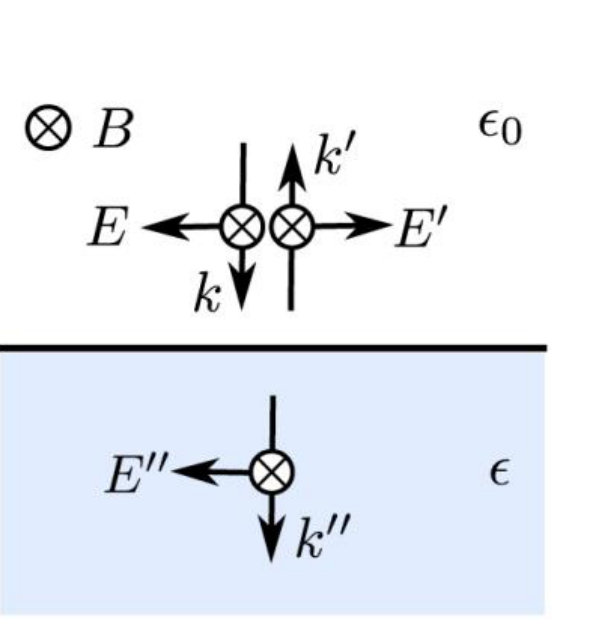
\includegraphics[width=\linewidth]{sample_normal_wave.png}
\end{column}
\end{columns}
$n=1.50$ 时 $r=-0.20$，$t=0.80$，$R=0.04$，$T=0.96$。透射电场是入射的 $0.8$ 倍，透射能量占 $96\%$，因为介质一侧的波阻抗更小。
\src{样卷第5题(1)(2)；缪讲义介质表面。无损介质。}
\end{frame}

\begin{frame}{导体中的电磁波-震荡模型}
均匀导体里，正离子不动。忽略碰撞和回复力时，自由电子数密度为 $N$，电场 $E=E_0\cos\omega t$ 使电子的位移为
\[
 x=\frac{eE}{m_e\omega^2}.
\]
极化强度 $P=-Nex$，于是
\[
 \boxed{\varepsilon(\omega)
 =\epso\!\left(1-\frac{\omega_p^2}{\omega^2}\right)},
 \qquad
 \omega_p=\sqrt{\frac{Ne^2}{\epso m_e}}.
\]
$\omega>\omega_p$ 时 $\varepsilon>0$，波可以传播。$\omega<\omega_p$ 时 $\varepsilon<0$，
\[
 k=\ii\kappa,\qquad
 \kappa=\frac{\sqrt{\omega_p^2-\omega^2}}{c}.
\]
电场在表面内按 $\e^{-\kappa z}$ 衰减，磁场与电场相位差 $\pi/2$，平均能流为零。半无限厚又无碰撞时，能量反射率为 $1$。有碰撞时，低频导体以欧姆电导为主。
\src{缪讲义等离子体频率；样卷第5题(3)(4)。}
\end{frame}

\begin{frame}{导体中的电磁波-震荡模型}
金属电子数密度 $N=10^{28}\,\mathrm{m^{-3}}$，波长 $\lambda=500\,\mathrm{nm}$，金属占满半无限空间，仍忽略碰撞。
\[
 \omega_p=\sqrt{\frac{Ne^2}{\epso m_e}}
 =5.64\times10^{15}\unit{s^{-1}},
\]
\[
 \omega=\frac{2\pi c}{\lambda}
 =3.77\times10^{15}\unit{s^{-1}}.
\]
$\omega<\omega_p$，
\[
 \varepsilon_r=1-\frac{\omega_p^2}{\omega^2}\simeq-1.24,
 \qquad
 \kappa\simeq1.40\times10^{7}\unit{m^{-1}}.
\]
场在大约 $1/\kappa=72\unit{nm}$ 内衰减，能量反射率 $R=1$。这束绿光被金属全反射，没有净能流进入金属深处。

判断顺序是：先比较 $\omega$ 和 $\omega_p$，再看 $\varepsilon$ 的符号。$\varepsilon<0$ 时 $k$ 为虚数，无碰撞的半无限金属把入射能量全部反射。
\src{样卷第5题(4)。$e=1.60\times10^{-19}\unit{C}$，$m_e=9.11\times10^{-31}\unit{kg}$，$\epso=8.85\times10^{-12}\,\mathrm{F\,m^{-1}}$。}
\end{frame}

\begin{frame}{导体中的电磁波-电导模型}
导体里更常用的做法是直接写 $\vct J=\sigma\vct E$。单色场取 $\e^{-\ii\omega t}$ 时，
\[
 \nabla\times\vct H=\sigma\vct E-\ii\omega\varepsilon\vct E,
 \qquad
 \nabla\times\vct E=\ii\omega\mu\vct H.
\]
消去 $\vct H$。均匀导体内部 $\nabla\cdot\vct E=0$，得到亥姆霍兹方程
\[
 \boxed{\nabla^2\vct E+k^2\vct E=0},
 \qquad
 k^2=\mu\varepsilon\omega^2+\ii\mu\sigma\omega.
\]
也可写成 $k^2=\mu\varepsilon_c\omega^2$，$\varepsilon_c=\varepsilon+\ii\sigma/\omega$。$\sigma$ 是给定的常数，不需要再从电子运动求介电函数。

良导体 $\sigma\gg\omega\varepsilon$ 时，$k^2\approx\ii\mu\sigma\omega$，
\[
 k=\frac{1+\ii}{\delta},\qquad
 \delta=\sqrt{\frac{2}{\mu\sigma\omega}}.
\]
沿 $+z$ 传播的场按 $\e^{-z/\delta}$ 衰减。$\delta$ 是趋肤深度。$\sigma$ 越大、频率越高，波进入导体越浅。
\src{由 $\vct J=\sigma\vct E$ 代入安培--麦克斯韦方程。时间因子为 $\e^{-\ii\omega t}$。}
\end{frame}

\begin{frame}{发射功率}
某广播电台希望在 $100\,\mathrm{km}$ 外，信号电场的振幅不小于 $0.10\,\mathrm{V\,m^{-1}}$。求发射功率至少要多大。

按真空、各方向发射相同、没有传播损耗来估计。远处一小块波面用平面波的平均能流 \(I=E_0^2/(2Z_0)\)。

Z0是真空波阻抗的数值。由 \(c=1/\sqrt{\muo\epso}\)，
\[
 Z_0=\sqrt{\frac{\muo}{\epso}}=\muo c.
\]
取 \(\muo=4\pi\times10^{-7}\)、\(c=3.00\times10^{8}\)，得到 \(Z_0=120\pi\simeq377\,\Omega\)。

这些功率铺在半径 $r$ 的整个球面上，
\[
 \boxed{P_{\min}=4\pi r^2 I
 =\frac{2\pi r^2 E_0^2}{Z_0}
 \simeq1.67\times10^{6}\,\mathrm{W}}.
\]
距离加倍，或要求的振幅加倍，功率都变为四倍。
\src{张讲义习题9.3。}
\end{frame}

\begin{frame}[plain]
\centering
\vspace*{\fill}
{\fontsize{36}{48}\selectfont\color{courseblue}祝同学们考试顺利！\par}
\vspace{0.85cm}
{\large Weiyang College, Tsinghua University\par}
\vspace{0.22cm}
Steven.s\par
\vspace*{\fill}
\end{frame}
\end{document}
